% Pengaturan ukuran teks dan bentuk halaman dua sisi
\documentclass[12pt]{book}

% Pengaturan ukuran halaman dan margin
\usepackage[a4paper,top=30mm,left=30mm,right=20mm,bottom=25mm]{geometry}

% Pengaturan ukuran spasi
\usepackage[singlespacing]{setspace}

% Pengaturan caption untuk tabel
\usepackage{caption}

% Judul dokumen
\title{Proposal Tugas Akhir ITS}
\author{Samawi, Taib Izzat}

% Pengaturan detail pada file PDF
\usepackage[pdfauthor={\@author},bookmarksnumbered,pdfborder={0 0 0}]{hyperref}


% Pengaturan ukuran indentasi
\setlength{\parindent}{2em}

% Package lainnya
\usepackage{changepage}
\usepackage{etoolbox} % Mengubah fungsi default

% Pengaturan jenis karakter
\usepackage{fontspec}

\usepackage[style=apa, backend=biber]{biblatex}
\usepackage{enumitem} % Pembuatan list
\usepackage{lipsum} % Pembuatan template kalimat
\usepackage{graphicx} % Input gambar
\usepackage{longtable} % Pembuatan tabel
\usepackage[table,xcdraw]{xcolor} % Pewarnaan tabel
\usepackage{eso-pic} % Untuk menggunakan background image di halaman
\usepackage{amsmath}
\setmainfont{Times New Roman}
\setsansfont{Arial}
\usepackage{changepage} % Pembuatan teks kolom
\usepackage{multicol} % Pembuatan kolom ganda
\usepackage{multirow} % Pembuatan baris ganda
\usepackage{tabularx} % Untuk mengatur kolom, seperti grid pada CSS
\usepackage{wrapfig}
\usepackage{float}
\floatplacement{algorithm}{H}

\usepackage{changepage}
\usepackage{enumitem}
\usepackage{eso-pic}
\usepackage{diagbox}
% \usepackage{txfonts} % Font times
\usepackage{etoolbox}
\usepackage{graphicx}
\usepackage{lipsum}
\usepackage{longtable}
\usepackage{tabularx}
\usepackage{wrapfig}
\usepackage{float}

% ini custom punya taib
\usepackage{booktabs}
\usepackage{algorithm}
\usepackage{algpseudocode}
% \usepackage{amsmath}

% Pengaturan format daftar isi, daftar gambar, dan daftar tabel
\usepackage[titles]{tocloft}
\setlength{\cftsecindent}{2em}
\setlength{\cftsubsecindent}{2em}
\setlength{\cftbeforechapskip}{1.5ex}
\setlength{\cftbeforesecskip}{1.5ex}
\setlength{\cftbeforetoctitleskip}{0cm}
\setlength{\cftbeforeloftitleskip}{0cm}
\setlength{\cftbeforelottitleskip}{0cm}
\renewcommand{\cfttoctitlefont}{\hfill\Large\bfseries} % command untuk membuat heading bold dan besar
\renewcommand{\cftaftertoctitle}{\hfill}
\renewcommand{\cftloftitlefont}{\hfill\Large\bfseries}
\renewcommand{\cftafterloftitle}{\hfill}
\renewcommand{\cftlottitlefont}{\hfill\Large\bfseries}
\renewcommand{\cftafterlottitle}{\hfill}

% Definisi untuk "Hati ini sengaja dikosongkan"
\patchcmd{\cleardoublepage}{\hbox{}}{
  \thispagestyle{empty}
  \vspace*{\fill}
  \begin{center}\textit{[This page is intentionally left blank]}\end{center}
  \vfill}{}{}

  % Pengaturan penomoran halaman
\usepackage{fancyhdr}
\fancyhf{}
\renewcommand{\headrulewidth}{0pt}
\pagestyle{fancy}
\fancyfoot[C,CO]{\thepage}
\patchcmd{\chapter}{plain}{fancy}{}{}
\patchcmd{\chapter}{empty}{plain}{}{}

% Pengaturan format judul bab
\usepackage{titlesec}
\renewcommand{\thesection}{\thechapter.\arabic{section}}
\titleformat{\chapter}[hang]{\centering\bfseries\large}{CHAPTER\ \arabic{chapter}\ }{0ex}{\vspace{0ex}\centering}
\titleformat*{\section}{\large\bfseries}
\titleformat*{\subsection}{\normalsize\bfseries}
\titlespacing{\chapter}{0ex}{0ex}{4ex}
\titlespacing{\section}{0ex}{1ex}{0ex}
\titlespacing{\subsection}{0ex}{0.5ex}{0ex}
\titlespacing{\subsubsection}{0ex}{0.5ex}{0ex}
\setcounter{secnumdepth}{3} % Untuk memberi penomoran pada \subsubsection

\counterwithin{figure}{chapter}
\counterwithin{table}{chapter}
\counterwithin{algorithm}{chapter}

\newfloat{eqfloat}{tbhp}{loe}[chapter]  % 'tbhp' are standard float placement options
\floatname{eqfloat}{Equation}

\captionsetup[eqfloat]{format=plain, labelfont=bf, textfont=normalfont, rule=false}

% Commands to define and print List of Equations
\newcommand{\listequationsname}{List of Equations}
\newcommand{\listequations}{%
  \listof{eqfloat}{\listequationsname}%
}
% Mengganti figure dan table menjadi gambar dan tabel
\renewcommand{\figurename}{Figure}
\renewcommand{\tablename}{Table}

\input{pustaka/tanda-hubung.tex}
% Atur variabel berikut sesuai namanya

% nama
\newcommand{\name}{Taib Izzat Samawi}
\newcommand{\authorname}{Samawi, Taib Izzat}
\newcommand{\nickname}{Taib}
\newcommand{\advisor}{Dini Adni Navastara, S.Kom., M.Sc.}
\newcommand{\coadvisor}{Dr. Rudy Dikairono, S.T., M.T.}
\newcommand{\examinerone}{Penguji I Belum Ditentukan}
\newcommand{\examinertwo}{Penguji II Belum Ditentukan}
\newcommand{\examinerthree}{Penguji III Belum Ditentukan}
\newcommand{\headofdepartment}{Ir. Ary Mazharuddin Shiddiqi, S.Kom., M.Comp.Sc., Ph.D}

% identitasr
\newcommand{\nrp}{5025221085}
\newcommand{\advisornip}{19851017 201504 2 001}
\newcommand{\coadvisornip}{19810325 200501 1 002}
\newcommand{\examineronenip}{18560710 194301 1 001}
\newcommand{\examinertwonip}{18560710 194301 1 001}
\newcommand{\examinerthreenip}{18560710 194301 1 001}
\newcommand{\headofdepartmentnip}{18810313 196901 1 001}

% judul
\newcommand{\tatitle}{\MakeUppercase{Real-Time Lidar-Inertial-Visual Odometry, Object Detection, and Mapping}}
\newcommand{\engtatitle}{\emph{\MakeUppercase{Real-Time Lidar-Inertial-Visual Odometry, Object Detection, and Mapping}}}

% tempat
\newcommand{\place}{Surabaya}

% jurusan
\newcommand{\studyprogram}{Teknik Informatika}
\newcommand{\engstudyprogram}{Informatics}

% fakultas
\newcommand{\faculty}{Teknologi Elektro dan Informatika Cerdas}
\newcommand{\engfaculty}{Intelligent Electrical and Informatics Technology}

% singkatan fakultas
\newcommand{\facultyshort}{FTEIC}
\newcommand{\engfacultyshort}{F-ELECTICS}

% departemen
\newcommand{\department}{Teknik Informatika}
\newcommand{\engdepartment}{Informatics}

% kode mata kuliah
\newcommand{\coursecode}{TD123456}


% Menambahkan resource daftar pustaka
\addbibresource{pustaka/pustaka.bib}

\raggedbottom

% Isi keseluruhan dokumen
\begin{document}
  % Nomor halaman pembuka dimulai dari sini
  \pagenumbering{roman}

  % Atur ulang penomoran halaman
  \setcounter{page}{1}

  % English Cover
  \newcommand\covercontents{sampul/konten-id.tex}
  \input{sampul/sampul-luar.tex}

  % Lembar pengesahan
  \chapter*{APPROVAL SHEET}

% Menyembunyikan nomor halaman
\thispagestyle{empty}

\begin{center}
  % Ubah kalimat berikut dengan judul tugas akhir
  \textbf{\tatitle}
\end{center}

\begingroup
% Pemilihan font ukuran small
\small

\begin{center}
  \textbf{FINAL PROJECT PROPOSAL} \\
  Submitted to fulfill one of the requirements for obtaining \\ 

  a Bachelor's Degree in Computer Science (\emph{Sarjana Komputer}) \\
  under the Undergraduate Study Program in Computer Science (\emph{Program Studi S-1 Teknik Informatika}) \\

  Department of \engdepartment{} \\
  Faculty of \engfaculty{} (F-ELECTICS) \\
  Institut Teknologi Sepuluh Nopember
\end{center}

\begin{center}
  % Ubah kalimat berikut dengan nama dan NRP mahasiswa
  By: \textbf{\name} \\
  NRP. \nrp
\end{center}

\begin{center}
  Approved by:
\end{center}

\vspace{10ex}

\begingroup
% Menghilangkan padding
\setlength{\tabcolsep}{0pt}

\noindent
\begin{tabularx}{\textwidth}{X c}
  % Ubah kalimat-kalimat berikut dengan nama dan NIP dosen pembimbing pertama
  \advisor      &                 \\
  NIP: \advisornip    & (Advisor)    \\
                                &                 \\
                                &                 \\
                                &                 \\
  % Ubah kalimat-kalimat berikut dengan nama dan NIP dosen pembimbing kedua
  \coadvisor &                 \\
  NIP: \coadvisornip    & (Co-Advisor) \\
\end{tabularx}
\endgroup

\vspace{\fill}

\begin{center}
  Acknowledged by,\\
  % Ubah kalimat berikut dengan nama departemen
  Head of the Department of \engdepartment{}, F-ELECTICS \\
  \vspace{10ex}
  % Ubah kalimat berikut dengan jabatan kepala departemen
  \underline{\headofdepartment{}.} \\
  NIP. \headofdepartmentnip{}\\
  \vspace{10ex}
  % Ubah text dibawah menjadi tempat dan tanggal
  \textbf{SURABAYA} \\
  \textbf{July 2025}
\end{center}
\endgroup

  \cleardoublepage

  % Abstrak
  \chapter*{ABSTRACT}
\begin{center}
  \large
  \textbf{\tatitle}
\end{center}
\addcontentsline{toc}{chapter}{ABSTRACT}
% Menyembunyikan nomor halaman
\thispagestyle{empty}

\begin{flushleft}
  \setlength{\tabcolsep}{0pt}
  \bfseries
  \begin{tabular}{ll@{\hspace{6pt}}l}
  Student Name / NRP&:& \name / \nrp\\
  Department &:& \engdepartment{} \engfacultyshort{} - ITS\\
  Advisors&:& 1. \advisor\\
  & & 2. \coadvisor\\
  \end{tabular}
  \vspace{4ex}
\end{flushleft}
\textbf{Abstract}

% Isi Abstrak

\sloppy
Advanced autonomous mobility is limited by the latency gap between environmental perception and action execution, especially in high-precision three-dimensional (3D) object detection systems. Current 3D detection models, despite being highly accurate, have a very high computational load and rely on non-real-time processing. This research addresses these challenges by introducing a novel lightweight framework for Real-Time Lidar-Inertial-Visual Odometry, Object Detection, and Mapping (RT-LIVO2DM). By designing an architecture that synergistically integrates data from LiDAR, IMU, and visual camera sensors, RT-LIVO2DM is aimed at computational efficiency on resource-constrained embedded systems. Furthermore, the sensor integration presented by the RT-LIVO2DM framework can facilitate high-precision 3D environmental mapping with color data. The environmental mapping data presented by RT-LIVO2DM paves the way for sustainable research related to Level 4/5 autonomous systems. The system's performance is quantitatively evaluated using the Waymo Open Dataset to validate its accuracy, latency, and computational load performance compared to other methods. This research is expected to demonstrate the feasibility of a high-accuracy 3D perception system capable of operating within real-time constraints on autonomous platforms and provide access to the collection of information-rich driving environment data, bridging the implementation gap and paving the way for safer and more reliable Level 4/5 autonomous systems.

\vspace{2ex}
\noindent
\textbf{Keywords: \emph{Real-Time, 3D Object Detection, 3D Mapping, Autonomous Mobility, Sensor Fusion, LiDAR, IMU, Computer Vision}} 
  \cleardoublepage

  % proposed ar\chapter*{ABSTRACT}
\begin{center}
  \large
  \textbf{\tatitle}
\end{center}
% Menyembunyikan nomor halaman
\thispagestyle{empty}

\begin{flushleft}
  \setlength{\tabcolsep}{0pt}
  \bfseries
  \begin{tabular}{lc@{\hspace{6pt}}l}
  Student Name / NRP&: &\name / \nrp\\
  Department&: &\engdepartment \space \engfacultyshort - ITS\\
  Advisor&: &1. \advisor\\
  & & 2. \coadvisor\\
  \end{tabular}
  \vspace{4ex}
\end{flushleft}
\textbf{Abstract}

% Isi Abstrak
Advanced autonomous mobility is limited by the latency gap between environmental perception and action execution, especially in high-precision three-dimensional (3D) object detection systems. Current state-of-the-art (SOTA) 3D detection models, despite being highly accurate, have a very high computational load and rely on non-real-time processing. This research addresses these challenges by introducing \textbf{RT-LIVO2DM}, a novel lightweight framework for simultaneous and real-time 3D odometry and object detection. By designing an architecture that synergistically integrates data from LiDAR, IMU, and visual camera sensors, \textbf{RT-LIVO2DM} is aimed at computational efficiency on resource-constrained embedded systems. Furthermore, the sensor integration presented by the \textbf{RT-LIVO2DM} framework can facilitate high-precision 3D environmental mapping. The environmental mapping data presented by \textbf{RT-LIVO2DM} paves the way for sustainable research related to Level 4/5 autonomous systems. The system's performance is quantitatively evaluated using the Waymo Open Dataset to validate its accuracy, latency, and computational load performance compared to SOTA methods. This research is expected to demonstrate the feasibility of a high-accuracy 3D perception system capable of operating within real-time constraints on autonomous platforms and provide access to the collection of information-rich driving environment data, bridging the implementation gap and paving the way for safer and more reliable Level 4/5 autonomous systems.

\vspace{2ex}
\noindent
\textbf{Kata Kunci: \emph{Real-Time, 3D Object Detection, 3D Mapping, Autonomous Mobility, Sensor Fusion, LiDAR, IMU, Computer Vision}} 
  % \cleardoublepage

  \begin{spacing}{1.5}
    % Daftar isi
    \renewcommand*\contentsname{TABLE OF CONTENTS}
    \addcontentsline{toc}{chapter}{\contentsname}
    \tableofcontents
    \cleardoublepage

    % Daftar gambar
    \renewcommand*\listfigurename{LIST OF FIGURES}
    \addcontentsline{toc}{chapter}{\listfigurename}
    \listoffigures
    \cleardoublepage

    % Daftar tabel
    \renewcommand*\listtablename{LIST OF TABLES}
    \addcontentsline{toc}{chapter}{\listtablename}
    \listoftables
    \cleardoublepage

    \renewcommand*\listalgorithmname{LIST OF ALGORITHMS}
    \addcontentsline{toc}{chapter}{\listalgorithmname}
    \listofalgorithms
    \cleardoublepage

    % \renewcommand*\listequationsname{LIST OF EQUATIONS}
    % \addcontentsline{toc}{chapter}{\listequationsname}
    % \listequations
    % \cleardoublepage
  \end{spacing}

  % Nomor halaman isi dimulai dari sini
  \pagenumbering{arabic}

  % Konten pendahuluan
  \chapter{INTRODUCTION}

\section{Background}

% Ubah paragraf-paragraf berikut sesuai dengan latar belakang dari tugas akhir
\sloppy

Autonomous vehicles are rapidly evolving from experimental platform into commercially and operationally viable systems accross various domains in the likes of urban mobility, logistics, and industrial automation. Research for autonomous mobility have been recently demonstrated in Indonesia for both civilian~\parencite{icar_drl} and industrial~\parencite{brin2024autonomous} applications, indicating an increasing urgency for development in autonomous mobility systems. One crucial part or subsystem required for autonomous mobility is environmental perception. This includes the collection of high-level information from the surroundings of the vehicle through any means. The high-level informations from the perception system will be passed on to motion control or navigation algorithms to determine the best course of action for any given scenario.

The inevitable necessity for \emph{onboard} real-time perception systems in autonomous vehicles stems from safety and operational viability requirements. The ability to prevent the majority of traffic accidents, as suggested by various studies on collision avoidance systems \parencite{external_dp_av}, relies entirely on the vehicle's capability to make decisions within sub-second timeframes, outside of any reliance towards cloud-based or internet-based information, which might be hindered in remote locations or in air-gapped environments. In sectors such as mining or search and rescue (SAR) operations where network connectivity is unreliable, dependence on \emph{offboard} processing becomes a critical failure point. Perception systems that can run directly on vehicle hardware with limited resources is a crucial step towards Level 4/5 autonomy.

Current methods for 3D object detection based on LiDAR~\parencite{ma2023detzero} have pushed performance boundaries using complex voxel-based \emph{backbone} architectures and multi-frame temporal data aggregation. Although highly accurate, these approaches come with significant computational overhead. Processing latency in such models often exceeds several hundred milliseconds, requiring the use of powerful and energy-intensive GPU hardware in an \emph{offboard} paradigm. This methodology is acceptable for high-definition map (\emph{HD map}) generation but fails to meet the needs of real-time autonomous navigation, where object detection and path planning must happen continuously with low latency.

This research aims to directly address the onboard processing challenge by introducing \textbf{RT-LIVO2DM}: a new lightweight framework for \emph{\textbf{R}eal-\textbf{T}ime \textbf{L}idar-\textbf{I}nertial-\textbf{V}isual \textbf{O}dometry and \textbf{O}bject \textbf{D}etection}. The main contribution of this research is a computationally efficient architecture that synergistically fuses LiDAR point cloud data, inertial measurements, and computer vision imagery to simultaneously perform localization and object detection within strict real-time constraints. In contrast to \emph{offboard} approach provided by existing methods, RT-LIVO2DM is explicitly designed to be implemented on embedded systems, enabling high-precision 3D perception directly on autonomous agents.

RT-LIVO2DM shifts the focus towards better class differentiation, rather than expending unnecessary computational resources on determining the exact size, shape, and contour of detected objects. This approach is expected to yield lower bounding box dimensions accuracy whilst significantly increasing class differentiation accuracy and reducing inference latency. The novel environmental perception approach is expected to provide rich real-time information to be fed to motion control or navigation systems, allowing for better decision making under the strict temporal and computational restraints of edge computing in autonomous vehicles.

\section{Problem Statement}
Based on the background described, the research problems can be formulated as follows:
\begin{enumerate}[nolistsep]
    \item How can a computationally efficient sensor fusion architecture combining LiDAR, inertial, and visual inputs be designed to enable simultaneous 3D object detection and odometry within real-time processing constraints on embedded (\emph{onboard}) hardware?
    \item To what extent does the performance (precision, latency, and computational load) of the proposed architecture compare with existing methods that operate \emph{offboard}?
\end{enumerate}

\section{Scope and Limitations}

This research is limited to the following scope:
\begin{enumerate}[nolistsep]
    \item The study focuses on the development and evaluation of the software architecture. Hardware design or sensor integration on a physical platform is not included.
    \item Sensor fusion is limited to LiDAR (point cloud), IMU (inertial measurement unit), and a monocular camera. Other sensors such as radar or GPS are not utilized.
    \item Quantitative performance evaluation is conducted \emph{offline} using the \emph{Waymo Open Dataset}, serving as a standard benchmark against other existing methods.
    \item The primary evaluation metrics are 3D object detection accuracy and per-frame processing latency on NVIDIA Jetson AGX ORIN hardware.
\end{enumerate}

\section{Objectives}
To address the above problem statements, this research has the following objectives:

\begin{enumerate}[nolistsep]
    \item To design and implement \textbf{RT-LIVO2DM}, a new lightweight framework architecture for real-time odometry and 3D object detection.
    \item To quantitatively evaluate the accuracy of RT-LIVO2DM against existing methods using \emph{precision} and \emph{inference time} metrics on the Waymo Open Dataset.
\end{enumerate}

\section{Benefits}
The results of this research are expected to provide the following benefits:
\begin{enumerate}
    \item Contribute a new architecture (\textbf{RT-LIVO2DM}) that is efficient for real-time 3D perception, which can serve as a reference for developing high-performance autonomous systems with limited computing resources.
    \item Support the acceleration of safe and reliable autonomous technology deployment in various critical industry sectors (logistics, mining, public transport) by reducing latency and offboard processing dependencies.
    \item Enhance the capability and reputation of Institut Teknologi Sepuluh Nopember in the fields of robotics, artificial intelligence, and autonomous systems research.
\end{enumerate}

  \cleardoublepage

  % Konten tinjauan pustaka
  \chapter{LITERATURE REVIEW}

% Modify the following contents according to the literature review
\section{Previous Research and Designs}
\subsection{DetZero}
DetZero \parencite{ma2023detzero} is a LiDAR-based 3D object detection framework that introduces a \emph{long-term scene flow} approach. Instead of relying on only one or a few frames of LiDAR data, DetZero analyzes a long sequence of data. Although highly accurate, its reliance on long sequential LiDAR data results in very high latency and non-\emph{real-time} performance. DetZero employs \emph{batch processing} rather than \emph{stream processing}, which makes it completely unsuitable for \emph{real-time} decision-making within fractions of a second. Figure~\ref{fig:detzero_arch} shows the architecture of DetZero.

\begin{figure}[H]
  \centering
  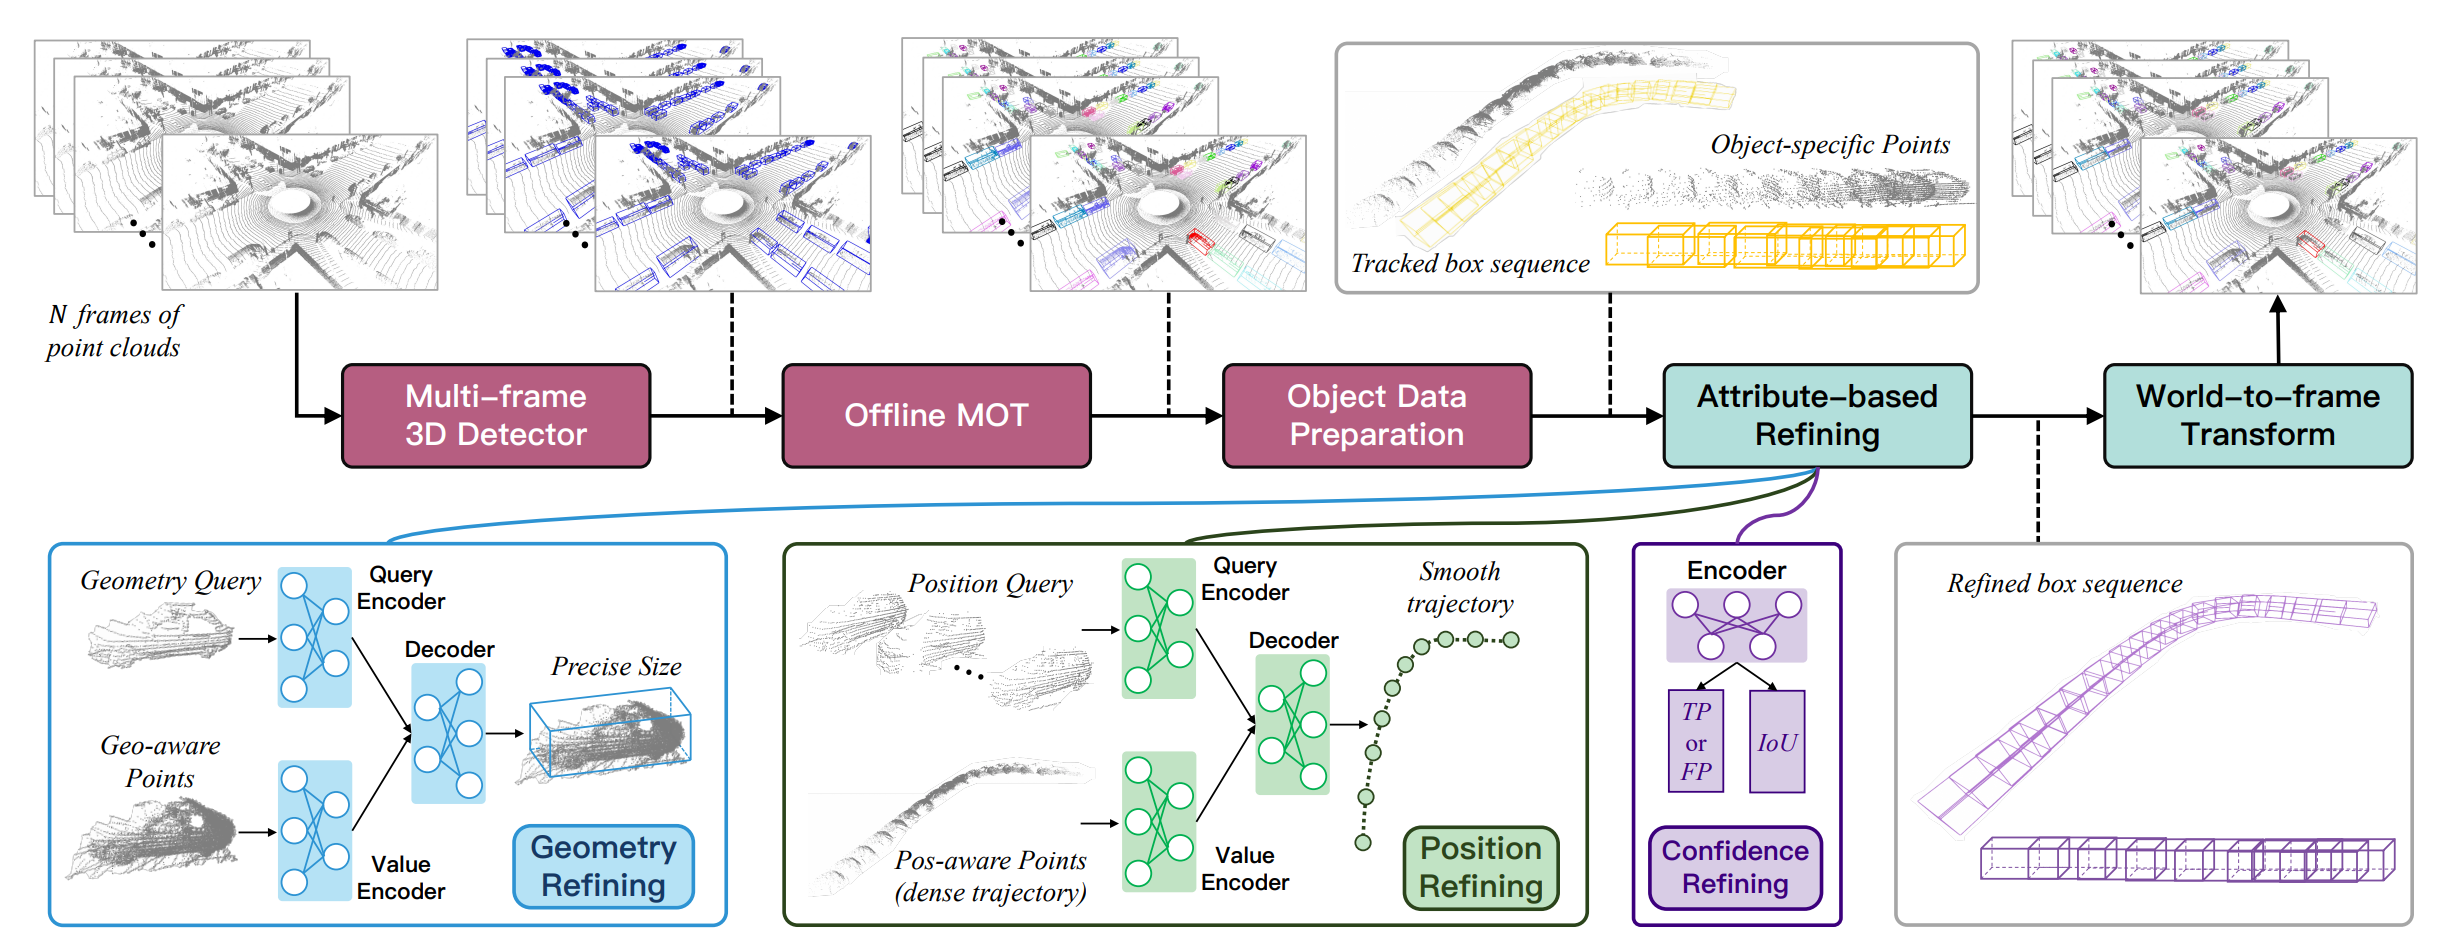
\includegraphics[scale=0.18]{gambar/detzero_architecture.png}
  \caption{DetZero System Architecture. DetZero introduces a multi-frame detector which aids in enhancing object point cloud geometry and detection quality.}
  \label{fig:detzero_arch}
\end{figure}

\subsection{PV-RCNN}
PV-RCNN converts the \emph{point cloud} into a series of 3D \emph{voxels} and applies 3D convolutional networks to extract features from the entire scene~\parencite{pvrcnn}. Figure~\ref{fig:pvrcnn_arch} shows the architecture of PV-RCNN. Essentially, PV-RCNN aims to perform in 3D what YOLO frameworks do in 2D. The major drawback of PV-RCNN lies in the voxelization step (transforming point clouds into 3D voxels/pixels), which consumes substantial computational resources. Additionally, PV-RCNN relies solely on the shape of an object to determine its class, which can lead to misclassifications between similarly shaped objects that differ significantly in color.

\begin{figure}[H]
  \centering
  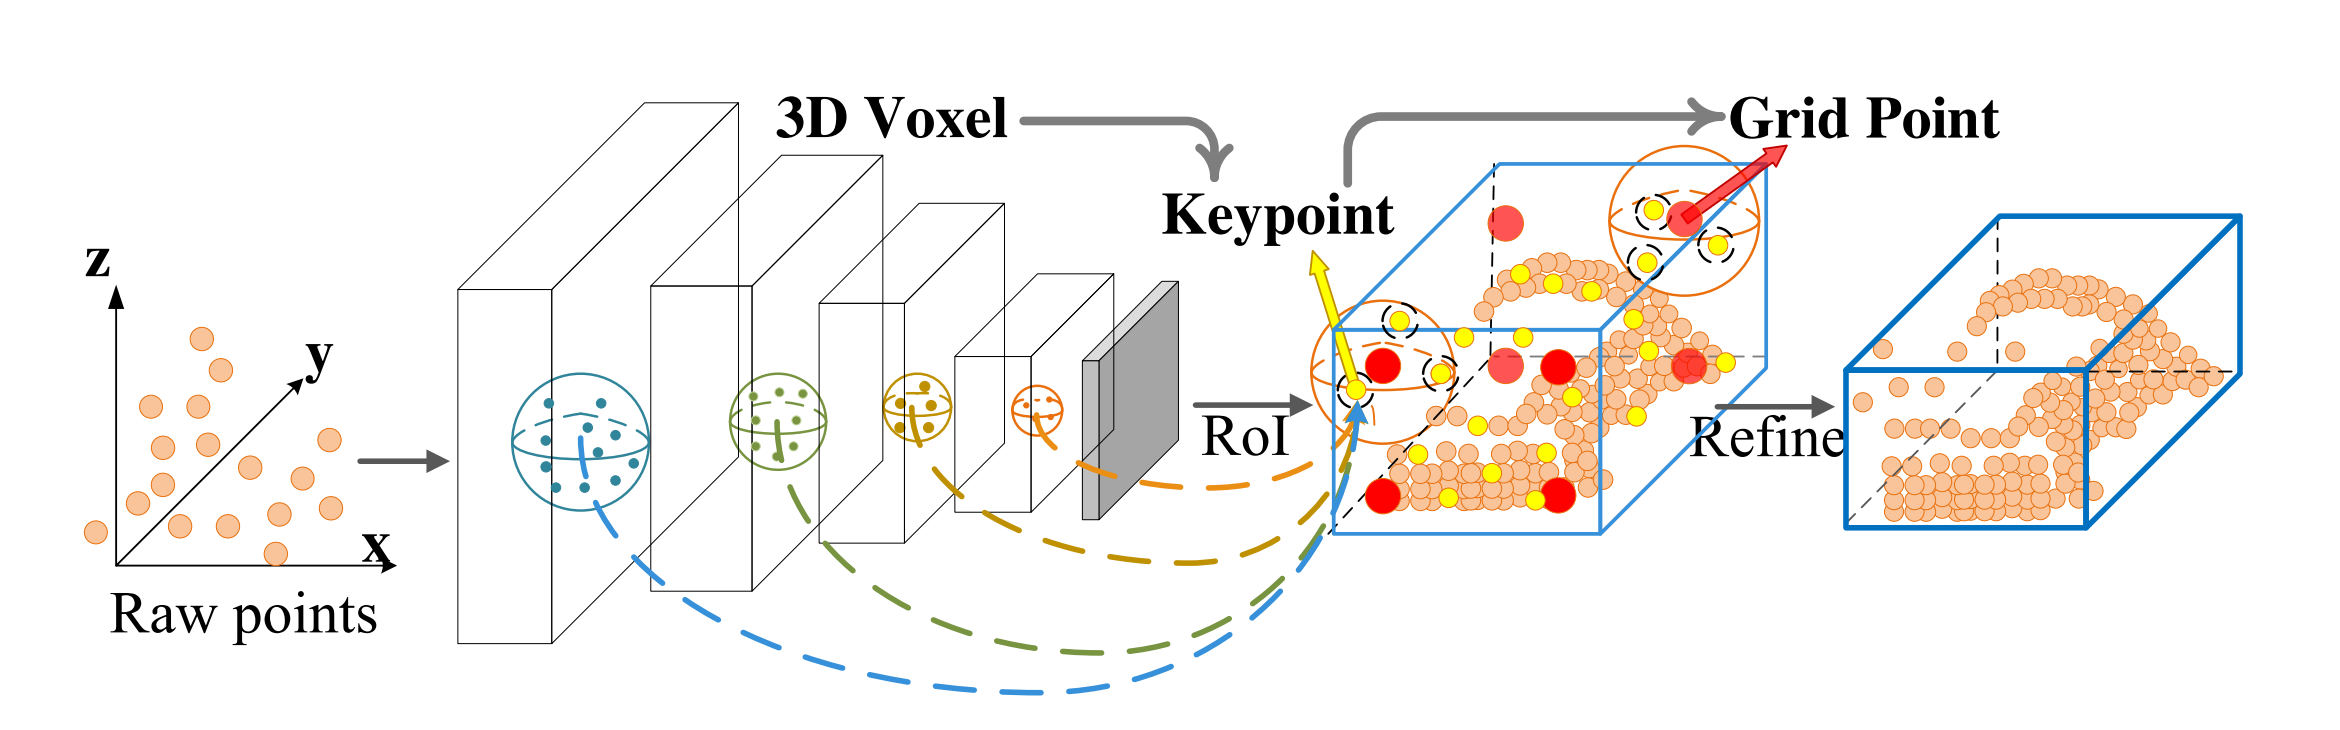
\includegraphics[scale=0.19]{gambar/pvrcnn_architecture.png}
  \caption{PV-RCNN System Architecture. PV-RCNN uses a voxel-to-keypoint 3D scene encoding to improve LiDAR-based 3D object detection.}
  \label{fig:pvrcnn_arch}
\end{figure}

\subsection{CenterPoint}
CenterPoint~\parencite{centerpoint} is an object detection framework that simplifies the detection head by predicting an \emph{objectsness heat-map} at the center of each instance, followed by a regression of size, yag, and velocity (a 3D modification of the anchor-box approach of YOLO versions up to YOLOv5). The absence of anchors reduces hyper-parameters and accelerates post-processing. CenterPoint employs a VoxelNet backbone with circular NMS and a 0.1m voxel grid, achieving 76.7 mAPH on Waymo LEVEL\_2, yet it needs 8 GB of GPU RAM plus 400 MB of CPU RAM and still takes 60 ms on an RTX-2080Ti in single-sweep mode, comfortably under the 40ms soft-real-time threshold on a 15W SoC. Because it ingests only one LiDAR sweep at a time, the lact of temporal smoothing causes bounding boxes to flicker across frames, and by ignoring both camera and IMU data it remains sensitive to viewport changed and ego-motion drift. Figure~\ref{fig:centerpoint_arch} shows the architecture of CenterPoint.

\begin{figure}[H]
  \centering
  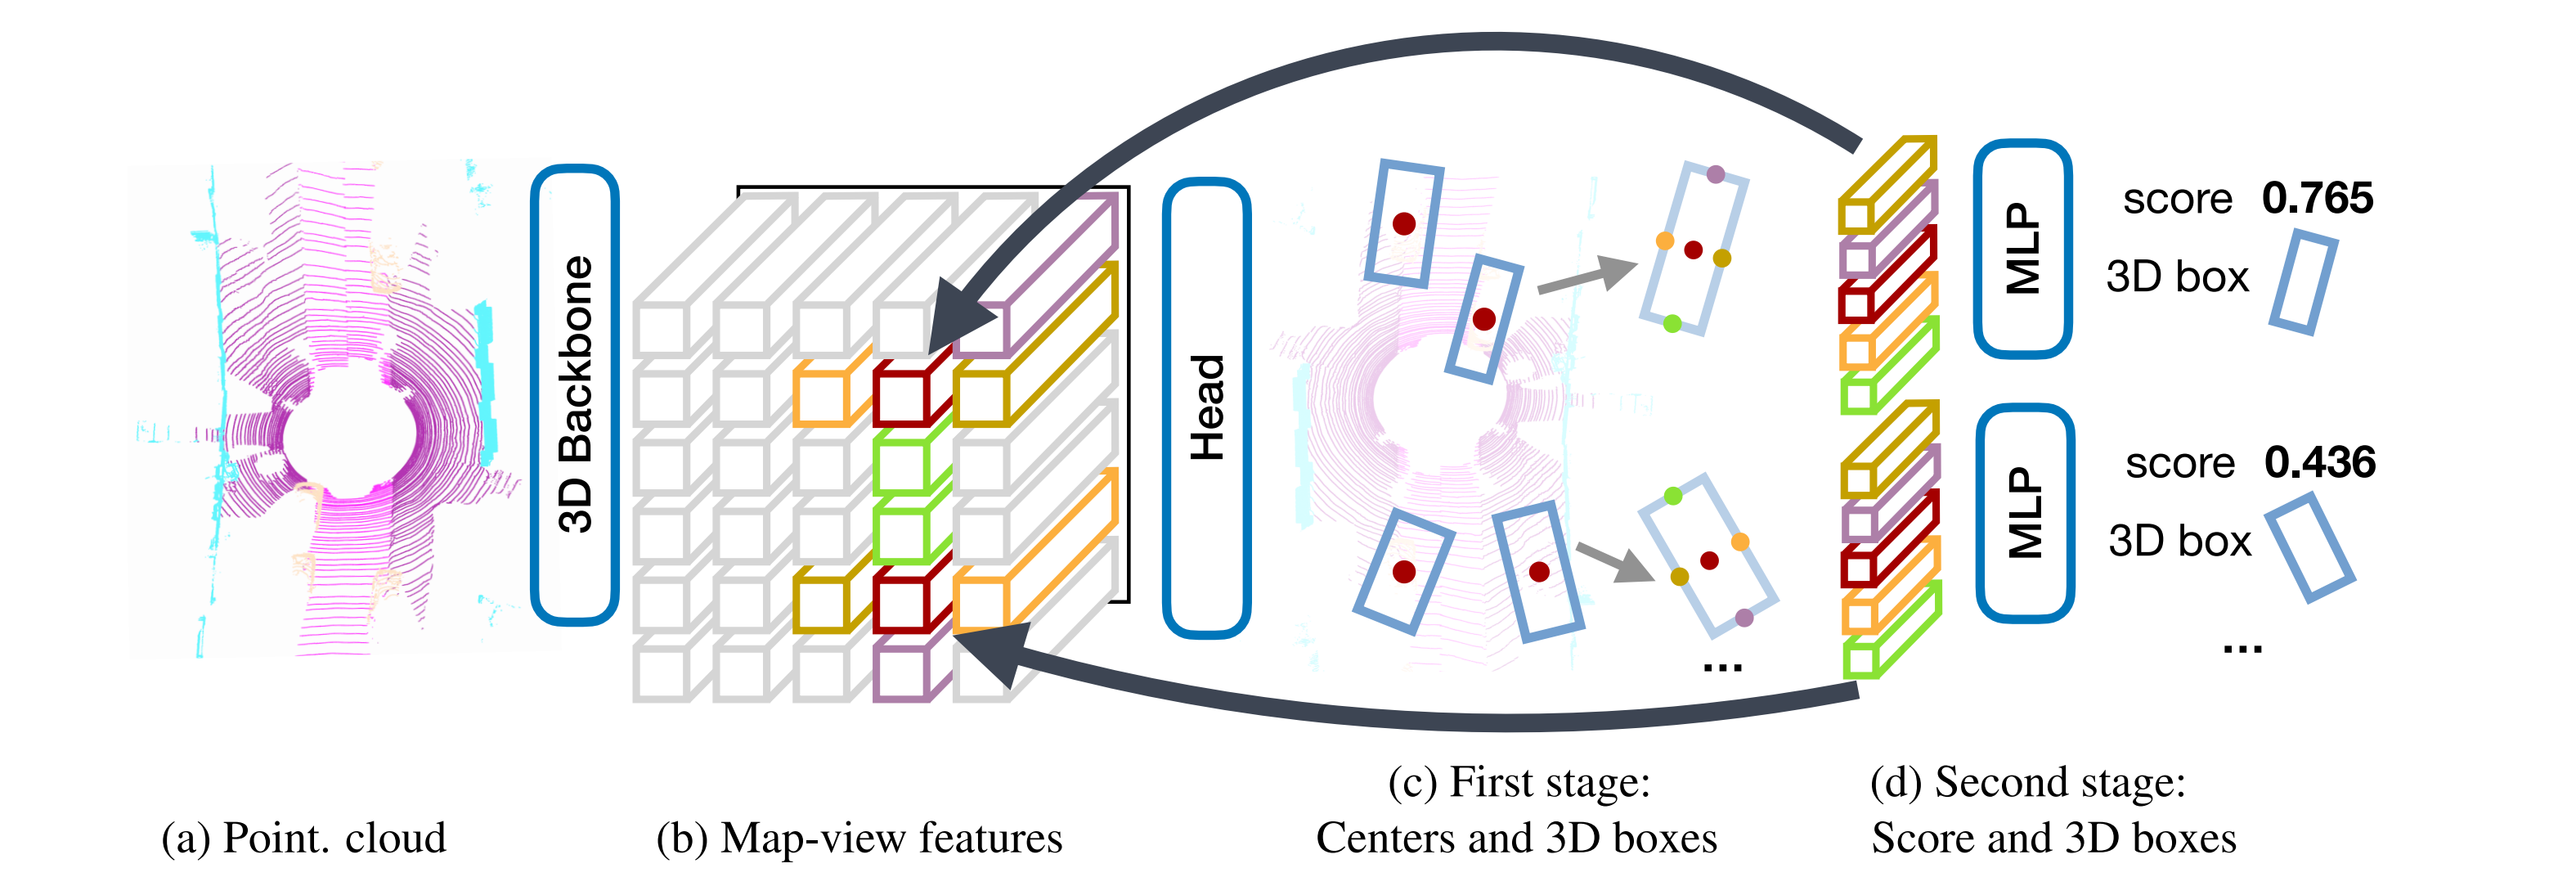
\includegraphics[scale=0.14]{gambar/centerpoint_architecture.png}
  \caption{CenterPoint System Architecture. CenterPoint uses a standard 3D backbone to extract features from LiDAR point clouds.}
  \label{fig:centerpoint_arch}
\end{figure}

\subsection{BEVFusion}
BEVFusion~\parencite{bevfusion} unifies camera and LiDAR features in a shared BEV raster by \emph{lifting} image features via predicted depth and then concatenating with LiDAR voxel features. Figure \ref{fig:dlio_arch} shows the architecture of BEVFusion. A shared transformer decoder refines the fused volume. BEVFusion ingests six 1920x1280 cameras plus one LiDAR sweep on the Waymo Open Dataset, relying on a dual-backbone that couples a Swin-T vision transformer with a VoxelNet LiDAR encoder and fuses their features thorugh deformable attention, achieving 78.9 mAPH on Waymo LEVEL\_2, but only after 120 ms on a pair of A100 GPUs that together drew about 200W. BEVFusion requires a power budget roughly two orders of magnitude beyond what an embedded SoC can spare, and the heavy transformer layers together with the dense bird's-eye-view (BEV) grid make on-device streaming impractical. Moveover, the system insists on six precisely calibrated cameras, locking users into a rigid sensor suite that complicates integration on smaller, more flexible autonomous platforms.

\begin{figure}[H]
  \centering
  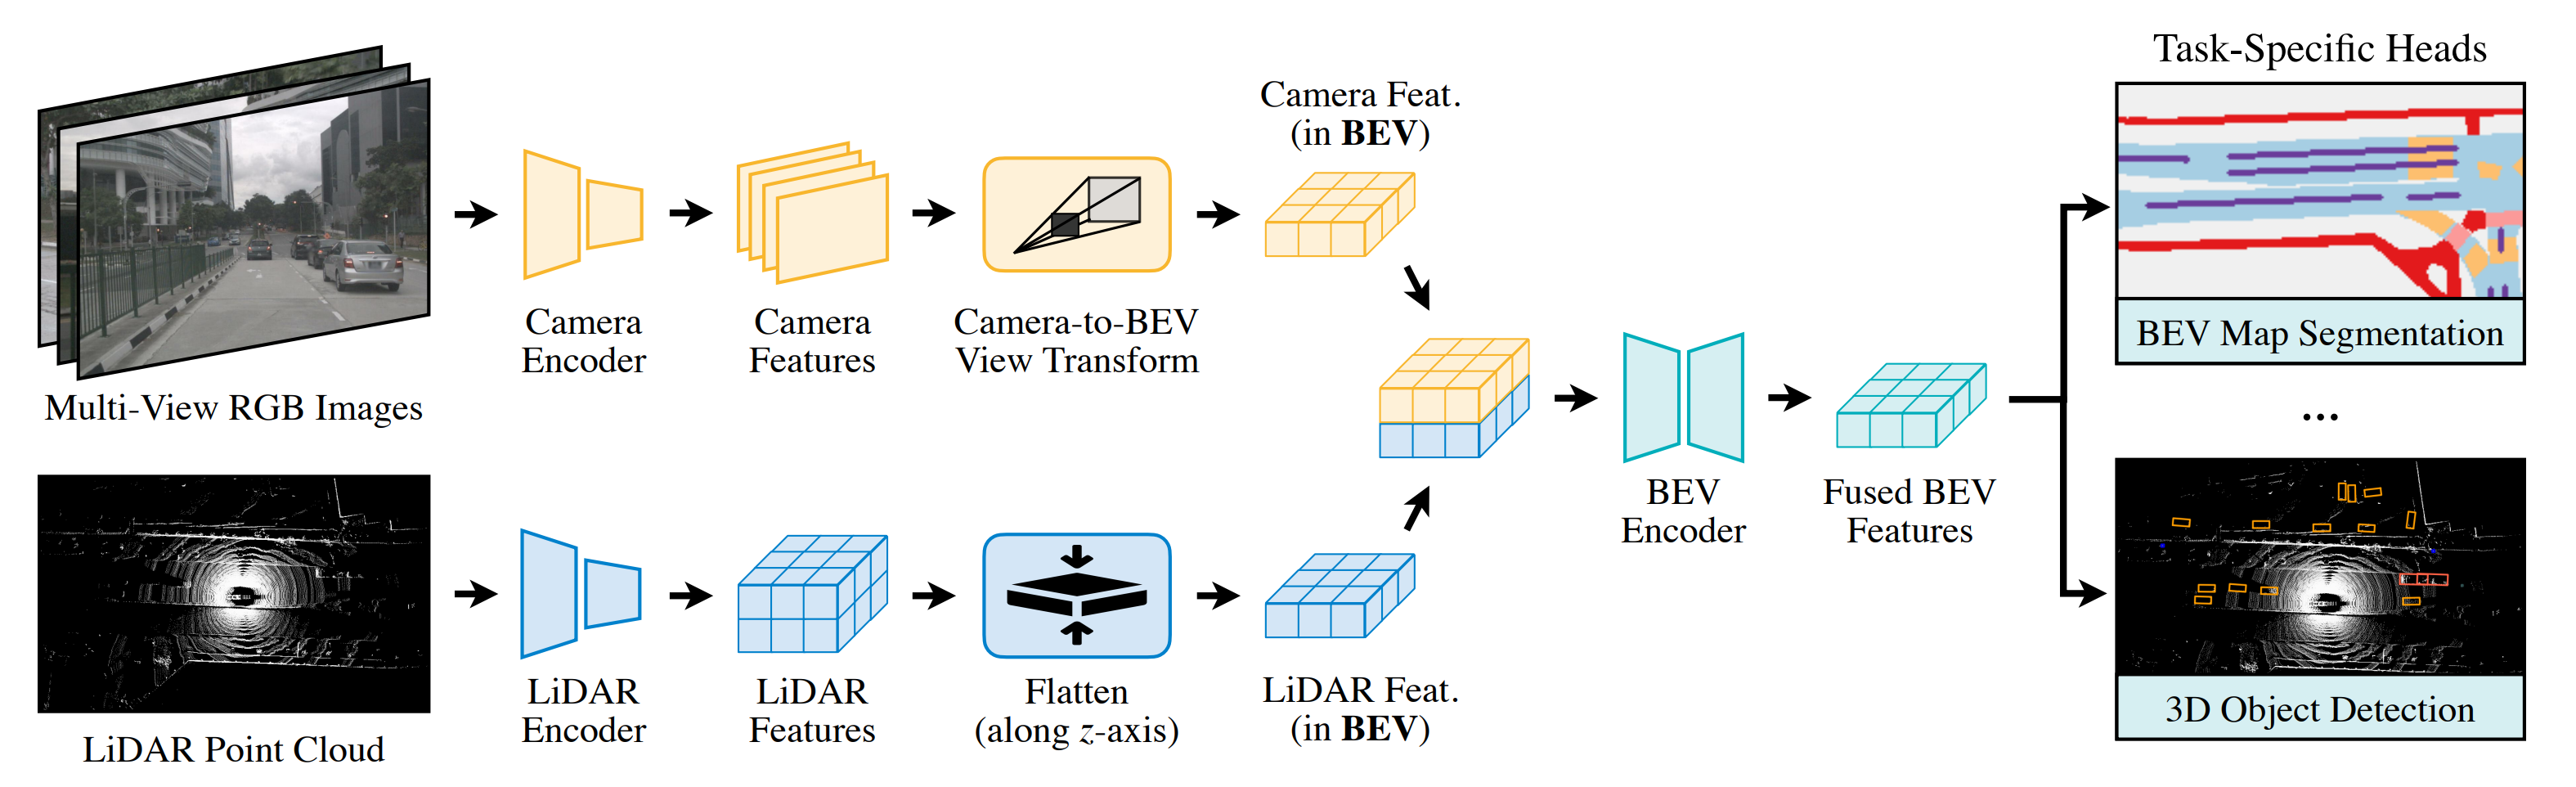
\includegraphics[scale=0.14]{gambar/bev_architecture.png}
  \caption{BEVFusion System Architecture. BEVFusion extracts camera and LiDAR features in a shared BEV raster by \emph{lifting} image features via predicted depth and then concatenating with LiDAR voxel features.}
  \label{fig:dlio_arch}
\end{figure}


\subsection{DLIO}
\emph{Direct LiDAR-Inertial Odometry} (DLIO) is an approach for ego-motion estimation, which is the process of determining the movement and orientation of a sensor (and the vehicle it is mounted on) over time. DLIO specifically combines data from a LiDAR sensor with data from an \emph{Inertial Measurement Unit} (IMU) to achieve accurate and robust trajectory estimation \parencite{dlio}. The word "Direct" in DLIO refers to the method used to process \emph{point cloud} data. Unlike "indirect" or feature-based methods, which first extract geometric features such as planes, edges, or corners from the \emph{point cloud} and then match these features across scans, the \emph{direct} method works directly on the raw point data. This method attempts to find the optimal transformation (rotation and translation) to align \emph{point clouds} from one time step to the next by directly minimizing geometric error. This approach avoids the feature extraction step, which can be computationally expensive and may discard useful information. Figure \ref{fig:dlio_viz} shows the architecture of DLIO.

\begin{figure}[H]
  \centering
  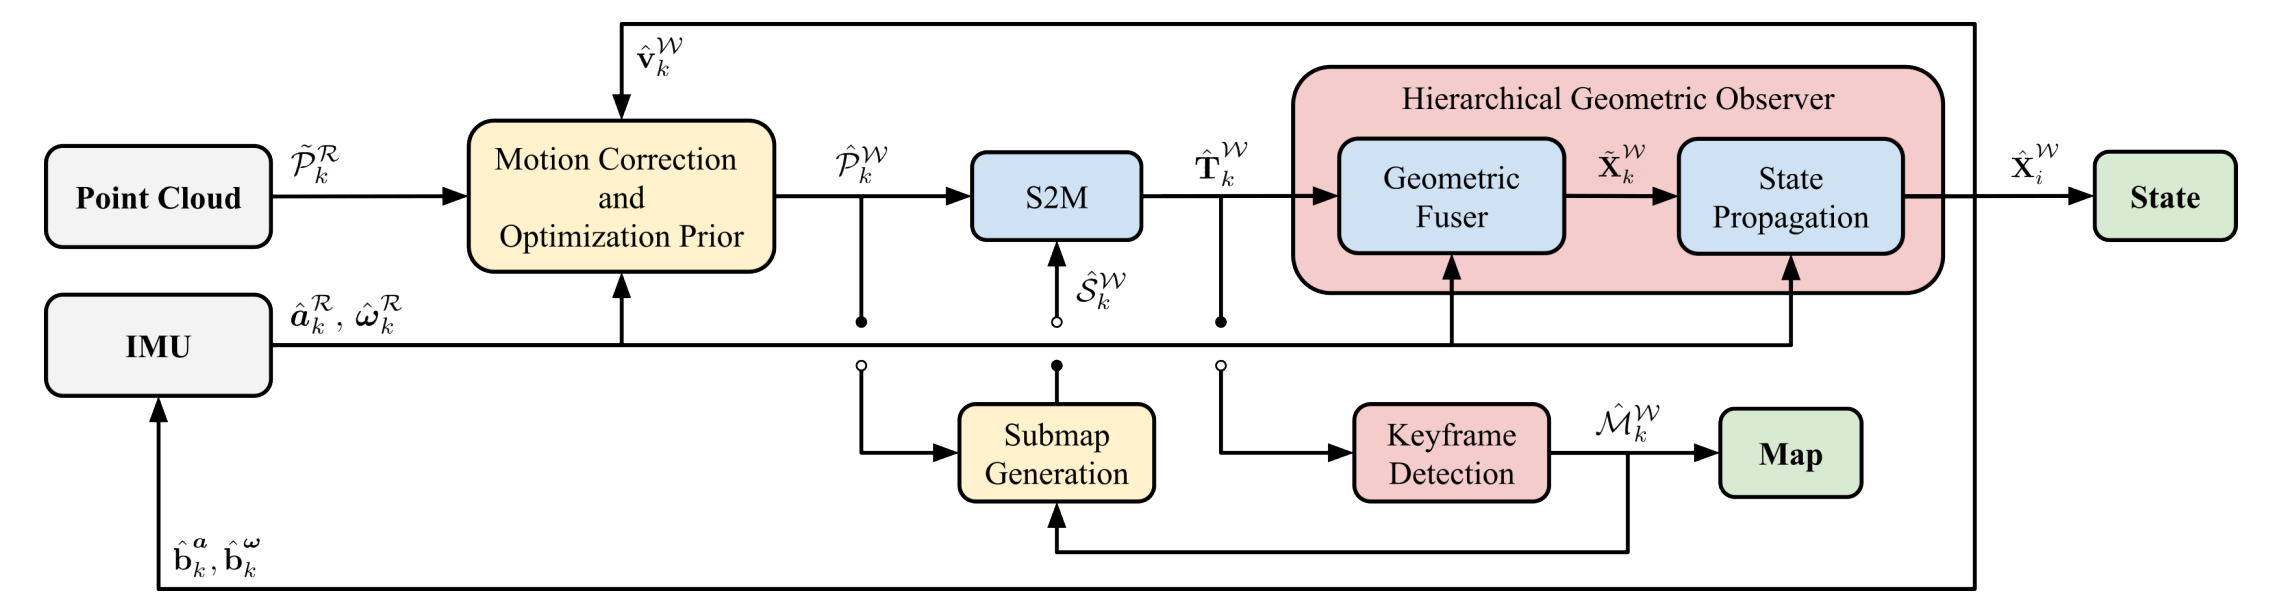
\includegraphics[scale=0.2]{gambar/dlio_architecture.png}
  \caption{DLIO System Architecture. DLIO provides a lightweight architecture that combines motion correction and prior construction into a single step, whilst also removing the computationally expensive scan-to-scan module previously required for LiDAR-based odometry.}
  \label{fig:dlio_viz}
\end{figure}

\subsection{Gap Analysis vs RT-LIVO2DM}

The following tables visualizes both the performance and qualitative gaps between each existing methods. Table~\ref{tab:gap_perf} lists mAPH on the Waymo Open Dataset validation split alongside latency and power, which highlights the divide between high-accuracy systems with hundreds of watts power requirement versus lightweight systems that sacrifice perception fidelity. Table~\ref{tab:gap_attrs} explains the major differences in sensor fusion and output attributes of each approach, with some methods relying on only LiDAR while others combine camera and LiDAR data, and some methods offer 3D maps while others do not.
% Table 1: Performance and Resource Footprint
\begin{table}[h!]
    \centering
    \caption{Gap Analysis: mAPH, Latency/FPS and Power}
    \begin{tabular}{lccc}
        \toprule
        \textbf{Method} & \textbf{mAPH} & \textbf{Latency / FPS} & \textbf{Power} \\
        \midrule
        DetZero     & 82.7 & 800 ms / 1.3 FPS & 300 W \\
        PV-RCNN     & 64.8 & 150 ms / 6.7 FPS & 250 W \\
        CenterPoint & 76.7 & 60 ms / 16 FPS  & 225 W \\
        BEVFusion   & 78.9 & 120 ms / 8 FPS  & 200 W \\
        DLIO        & —    & 8 ms / 125 FPS  & 45 W  \\
        \midrule
        \textbf{RT-LIVO2DM (Target)} & \textbf{$\geq 50$} & \textbf{$\leq 40$ ms / $\geq 25$ FPS} & \textbf{15--30 W} \\
        \bottomrule
    \end{tabular}
    \label{tab:gap_perf}
\end{table}

% Table 2: Sensor-Fusion & Output Capabilities
\begin{table}[h!]
    \centering
    \caption{Gap Analysis: Sensor Fusion and Output Attributes}
    \begin{tabular}{lccc}
        \toprule
        \textbf{Method} & \textbf{Color + IMU} & \textbf{Objects} & \textbf{3D Map} \\
        \midrule
        DetZero     & No  & Yes & Yes \\
        PV-RCNN     & No  & Yes & No  \\
        CenterPoint & No  & Yes & No  \\
        BEVFusion   & Yes & Yes & Yes \\
        DLIO        & Yes & No  & Yes \\
        \midrule
        \textbf{RT-LIVO2DM (Target)} & Yes & Yes & Yes, with Color \\
        \bottomrule
    \end{tabular}
    \label{tab:gap_attrs}
\end{table}

\section{Theoretical Foundations}

\subsection{LiDAR (\emph{Light Detection and Ranging})}

\begin{figure}[H]
  \centering
  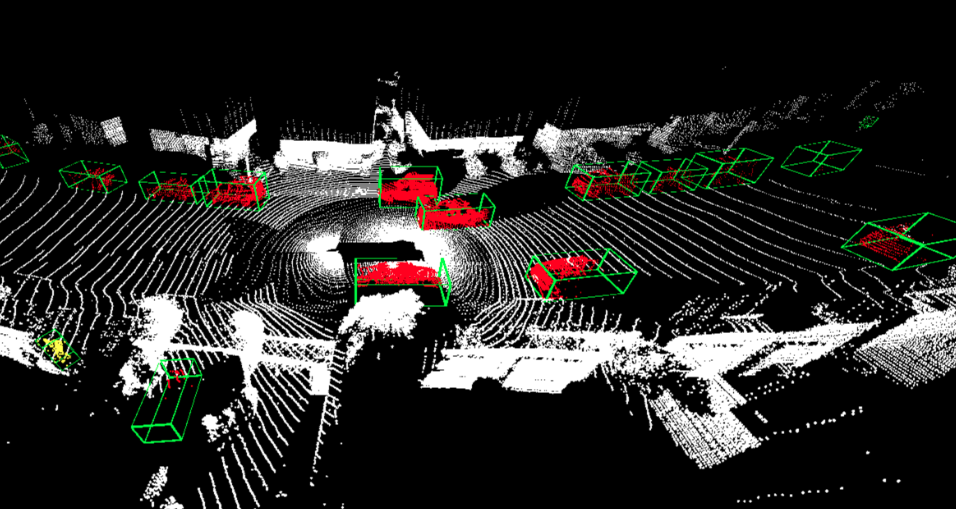
\includegraphics[scale=0.35]{gambar/waymo_lidar.png}
  \caption{Example of how LiDAR data is visualized, Waymo Open Dataset}
  \label{fig:waymo_lidar}
\end{figure}

LiDAR, short for \emph{Light Detection and Ranging}, is an active remote sensing method using pulsed laser light to measure distances from a fixed reference point~\parencite{lidar_principles}. It uses the \emph{time-of-flight} (ToF) principle (the same principle used in RADAR and SONAR systems), where a laser pulse (usually in infrared wavelength) is emitted toward an object and the time taken to return is used to determine the precise distance between the sensor and the object in which the light bounced on using the following equation:

\begin{equation}
  \label{eq:lidar_tof}
  d = \frac{c \cdot t}{2}
\end{equation}

Where:

\begin{itemize}
  \item $d$ is the distance to the object
  \item $c$ is the speed of light $ \approx 299.792 Km/s $
  \item $t$ is the round-trip time of the laser pulse
\end{itemize}

The data produced by LiDAR sensors is a collection of point data called a \emph{point cloud}, as shown in Figure~\ref{fig:waymo_lidar}. Each point in the \emph{point cloud} represents a single laser reflection and has 3D spatial coordinates (x, y, z). On some LiDAR devices, each point also carries additional information such as reflection intensity, which can help distinguish materials with different reflectivity. The main advantage of LiDAR compared to cameras is its ability to directly and accurately (without guesswork) measure depth, which can provide reliable information about 3D shapes and structures. Since LiDAR is a sensor that emits its own light source, its performance is not affected by external lighting conditions; LiDAR can function well at night as well as under bright sunlight.

Although it has advantages in 3D perception, LiDAR also has limitations in capturing rich color and texture information as a camera does. This makes it difficult to differentiate objects with similar shapes but different visual appearances (for example, a pedestrian and a traffic sign pole from certain angles). In addition, LiDAR performance can degrade significantly in weather conditions that produce many airborne particles such as very thick fog, rain, or snow.

\subsection{Computer Vision}
Like many AI implementations, developing a \emph{Computer Vision}-based system involves designing a \emph{model}—an algorithm that holds the foundational knowledge required to translate raw input into meaningful conclusions. A \emph{classifier} is the most suitable model type for object detection tasks, as it determines the object \emph{class} from given input data. The main goal of \emph{Computer Vision} implementation is to extract high-level information from images without human intervention. Applications include face recognition, motion detection in video, medical imaging, and more. Contemporary \emph{Computer Vision} approaches are dominated by \emph{Deep Learning} techniques~\parencite{deeplearning_lecun}, which continue to evolve rapidly at the time of writing.

% \emph{Deep Learning} (DL) adalah sebuah cabang dari \emph{Artificial Intelligence}/AI yang menggunakan jaringan saraf tiruan berlapis banyak (\emph{deep neural network}) untuk mempelajari representasi data. Efektivitas DL telah terdemonstrasi dalam beragam aplikasi, meliputi pengenalan citra, pemrosesan bahasa alami, dan deteksi objek.

\begin{figure}[H]
  \centering
  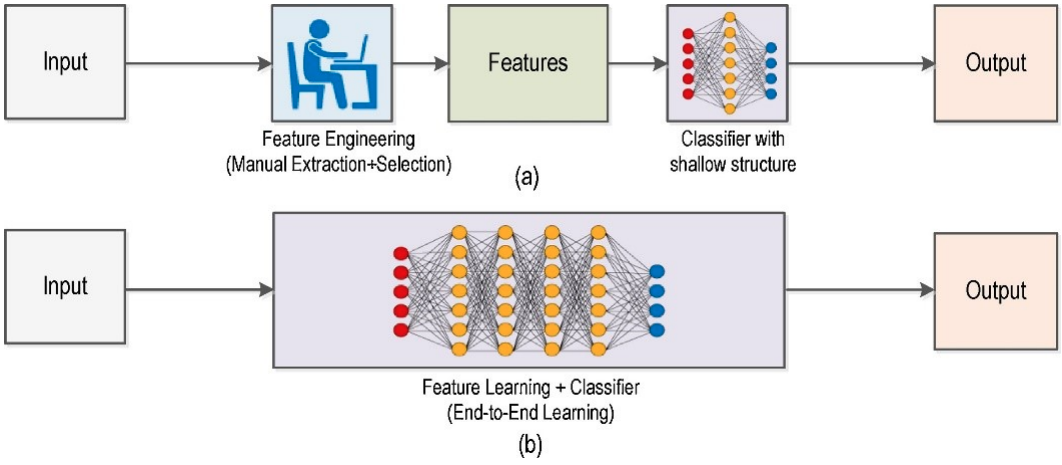
\includegraphics[scale=0.35]{gambar/traditional_vs_deep_learning_cv.png}
  \caption{(a) Traditional \emph{Computer Vision} approach vs. (b) \emph{Deep Learning}-based approach.}
  \label{fig:traditional_vs_deep_learning_cv}
\end{figure}

Visualized through Figure~\ref{fig:traditional_vs_deep_learning_cv}, before the advent of \emph{Deep Learning}, raw image data had to be manually interpreted into features (e.g., color, texture, shape) using \emph{Feature Selection} (FS) algorithms. Models then analyzed these features rather than raw pixels.

However, FS algorithm development was time-consuming, especially with many classes to detect. Moreover, adding a new class often required manual algorithm redesign. \emph{Deep Learning} automates FS by learning feature representations during training, enabling complex object detection and differentiation across hundreds of classes. AlexNet is commonly regarded as the first implementation that automates Feature Extraction with a Deep Convolutional Neural Network (DCNN)~\parencite{alexnet}.

\subsection{YOLO Framework}

YOLO (\emph{You Only Look Once}) is a \emph{Deep Learning}-based object detection algorithm designed for real-time performance. Instead of pinpointing exact object locations, it predicts \emph{confidence} values indicating the likelihood of objects in image regions \parencite{yolo_review}. Originally built for speed, newer YOLO versions have improved in accuracy and precision. Figure~\ref{fig:yolo_history} shows the development history of YOLO algorithms.

\begin{figure}[H]
  \centering
  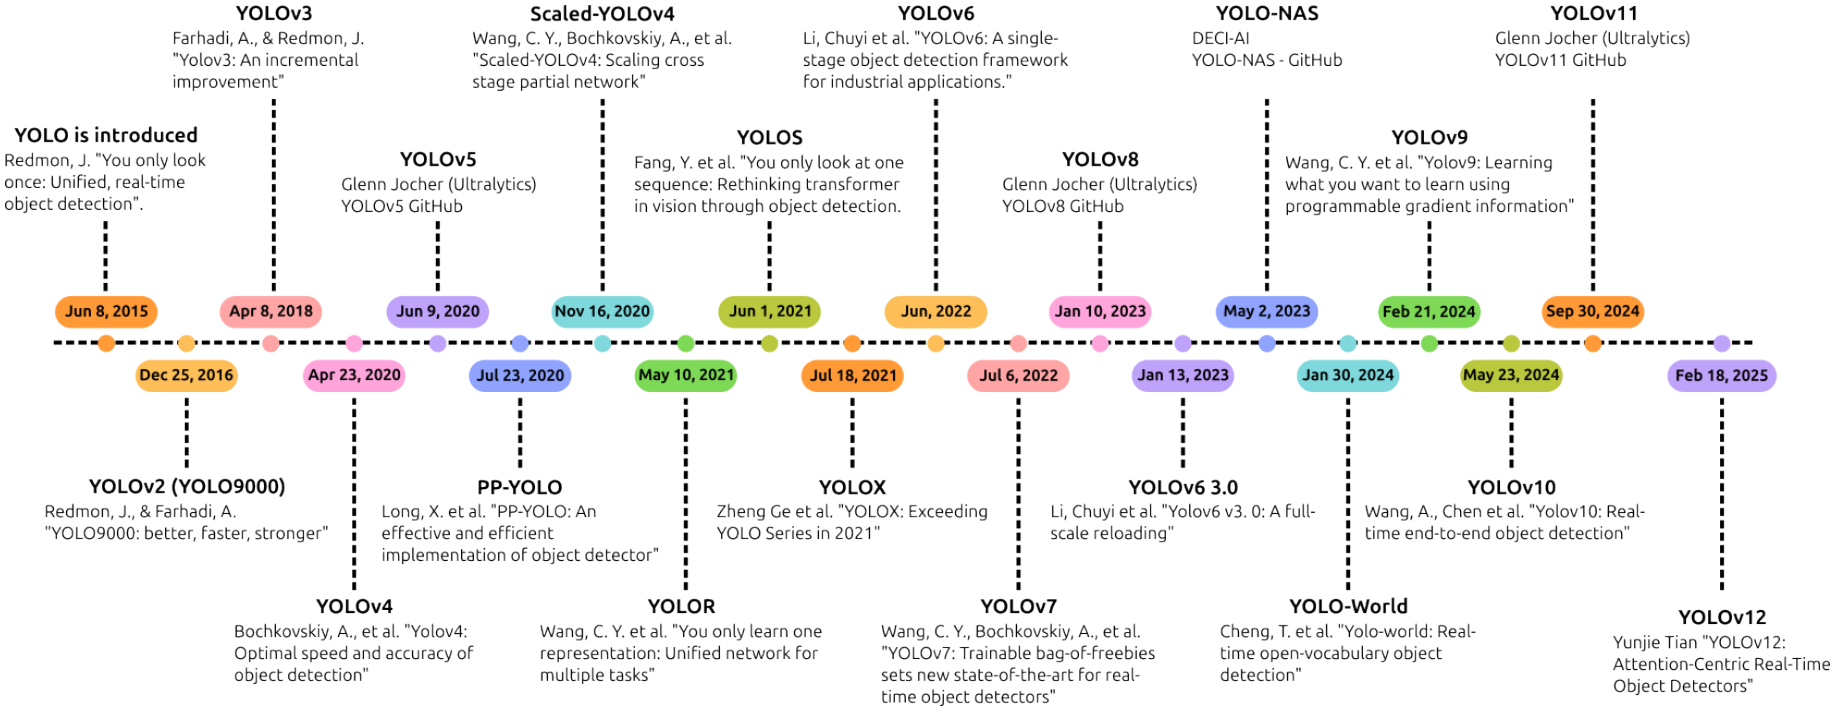
\includegraphics[width=\textwidth]{gambar/yolo_history.png}
  \caption{YOLO algorithm development history}
  \label{fig:yolo_history}
\end{figure}

Higher version numbers don't always indicate better performance. Some YOLO variants prioritize speed, others emphasize large-object detection, and some serve as experimental frameworks for new algorithmic techniques. Analysis shows YOLOv11 offers the best balance between accuracy and efficiency \parencite{yolo12_11_vs_others}. Ultralytics YOLOv11 is the latest version developed by Ultralytics. It improves both detection accuracy and inference speed over its predecessors. New features include multi-scale object detection, better small-object detection, and improved memory efficiency. Currently it is both more accurate and faster than the novel YOLOv12.

% \begin{figure}[H]
%   \centering
%   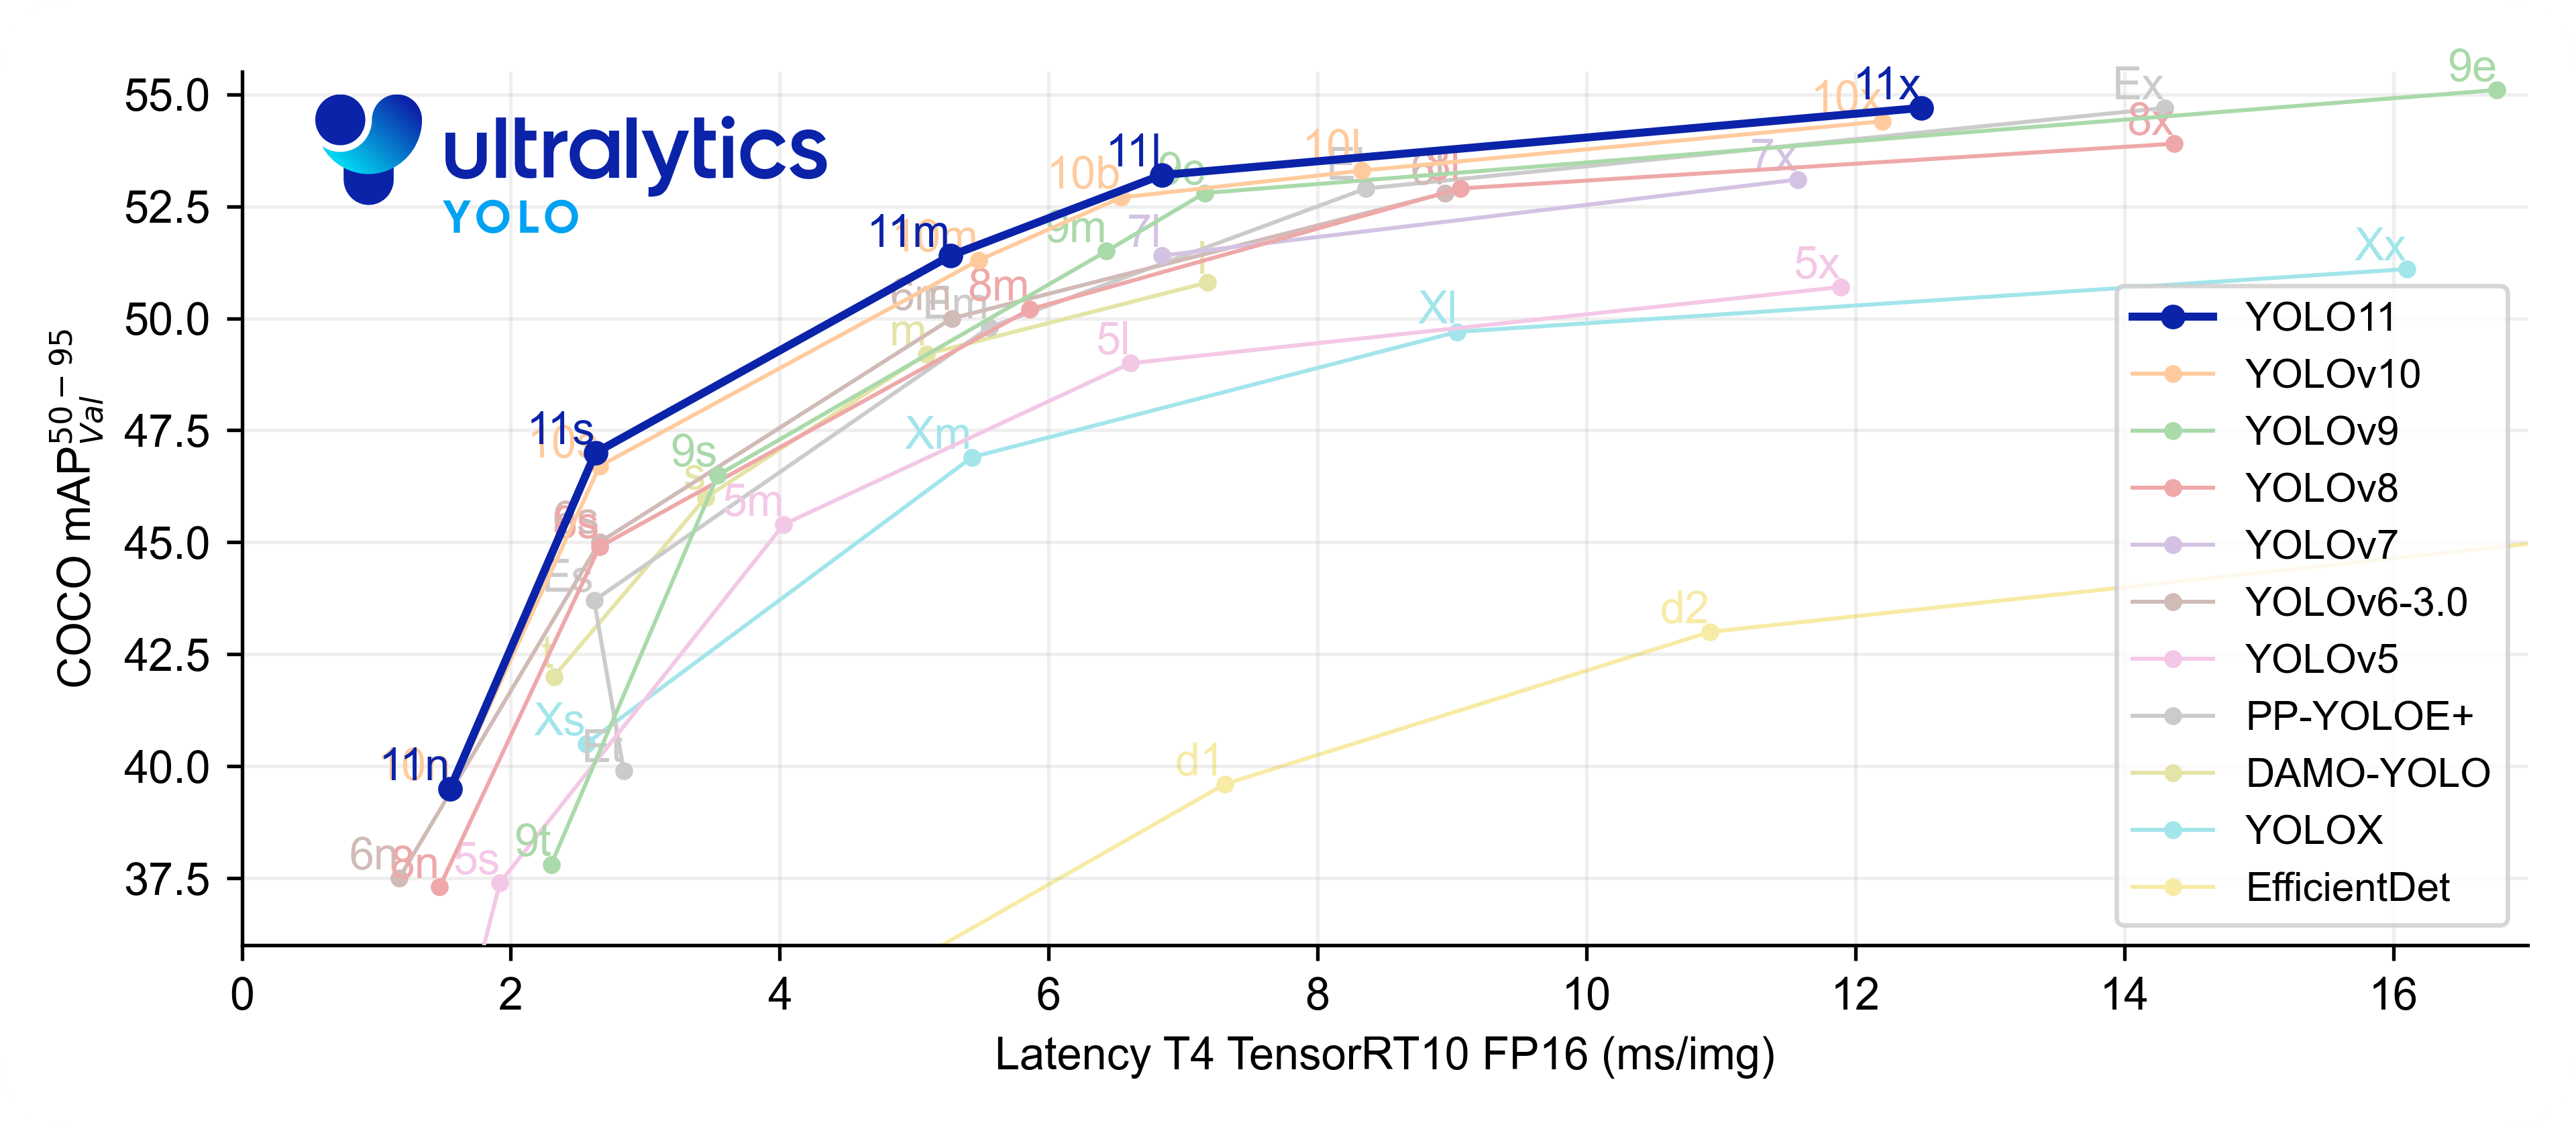
\includegraphics[width=\textwidth]{gambar/yolov11_performance.png}
%   \caption{YOLOv11 vs. other object detection algorithms \parencite{ultralytics2025yolo11}.}
%   \label{fig:yolov11_performance}
% \end{figure}

\subsection{Waymo Open Perception Dataset}

The Waymo Open Perception Dataset (WOPD) ~\parencite{Sun_2020_CVPR} is a publicly-available dataset provided by Waymo, an autonomous taxi company in the United States, a subsidiary of the Alphabet Group ~\parencite{waymo2025}. WOPD is a subset of the larger Waymo Open Dataset (WOD). WOPD is described as  having high resolution sensor data and labels for various tasks. The Waymo Open Perception Dataset is released through the official GitHub Repository~\parencite{waymo2025dataset}.

WOPD contains the following sensor data:

\sloppy
\begin{itemize}
    \item 1 mid-range LiDAR (\verb|T|)
    \item 4 short-range LiDARs (\verb|FRONT/F|, \verb|SIDE_LEFT/SL|, \verb|SIDE_RIGHT/SR|, \verb|REAR/R|)
    \item 5 cameras (\verb|FRONT/F|, \verb|FRONT_LEFT/FL|, \verb|FRONT_RIGHT/FR|, \verb|SIDE_LEFT/SL|, \verb|SIDE_RIGHT/SR|)
    \item Vehicle poses (\verb|IMU|)
\end{itemize}


Table~\ref{tab:wopd_full_specs_t} summarises the complete technical specification of every sensor and the pose attributes in the Waymo Open Perception Dataset.
Columns correspond to the five LiDAR units (TOP, F, SL, SR, R) and the five RGB cameras (F, FL, FR, SL, SR); the bottom block lists the synchronized 6-DoF vehicle pose, velocity, and global-timestamp auxiliary data that accompany every frame.

\begin{table}[h!]
  \centering
  \renewcommand{\arraystretch}{1.1}
  \small
  \caption{Transposed Sensor \& Pose Specifications. Values are taken from the official documentation for the Waymo Open Perception Dataset.}
  \label{tab:wopd_full_specs_t}
  \begin{tabular}{@{}lccccc@{}}
  \toprule
  \textbf{Attribute} & \textbf{T} & \textbf{F} & \textbf{SL} & \textbf{SR} & \textbf{R} \\ 
  \midrule
  \textbf{LiDAR} \\
  Beams & 64 & 16 & 16 & 16 & 16 \\
  Vertical Res. ($^\circ$) & 0.4 & 1.33 & 1.33 & 1.33 & 1.33 \\
  FOV (H × V) & 360 × 26.8 & 90 × 26.8 & 90 × 26.8 & 90 × 26.8 & 90 × 26.8 \\
  Range (m) & 0–75 & 0–20 & 0–20 & 0–20 & 0–20 \\
  Accuracy (cm) & $\pm$2 & $\pm$2 & $\pm$2 & $\pm$2 & $\pm$2 \\
  \midrule
  \textbf{Cameras (RGB)} & & & & & \\
  Resolution (px) & — & 1920×1280 & 1920×1280 & 1920×1040 & 1920×1040 \\
  HFOV ($^\circ$) & — & $\pm25.2$ & $\pm25.2$ & $\pm25.2$ & $\pm25.2$ \\
  VFOV ($^\circ$) & — & $\pm16.0$ & $\pm16.0$ & $\pm13.3$ & $\pm13.3$ \\
  \midrule
  \textbf{Pose / Auxiliary} \\
  Vehicle Pose & \multicolumn{5}{c}{6-DoF SE(3), position $\pm5$ cm, heading $\pm0.1^\circ$} \\
  Velocity & \multicolumn{5}{c}{3-DoF linear+angular, 10 Hz fused IMU/encoders} \\
  Timestamp & \multicolumn{5}{c}{64-bit µs, global clock $\le100$ µs error} \\
  \bottomrule
  \end{tabular}
\end{table}

Figure~\ref{fig:wopd_sensors} depicts the physical placement of these sensors on the roof-mounted mast, while Figure~\ref{fig:sensor_sync} quantifies the sub-millisecond hardware-level time alignment between LiDAR sweeps and camera exposures provided by WOPD.

\begin{figure}[H]
  \centering
  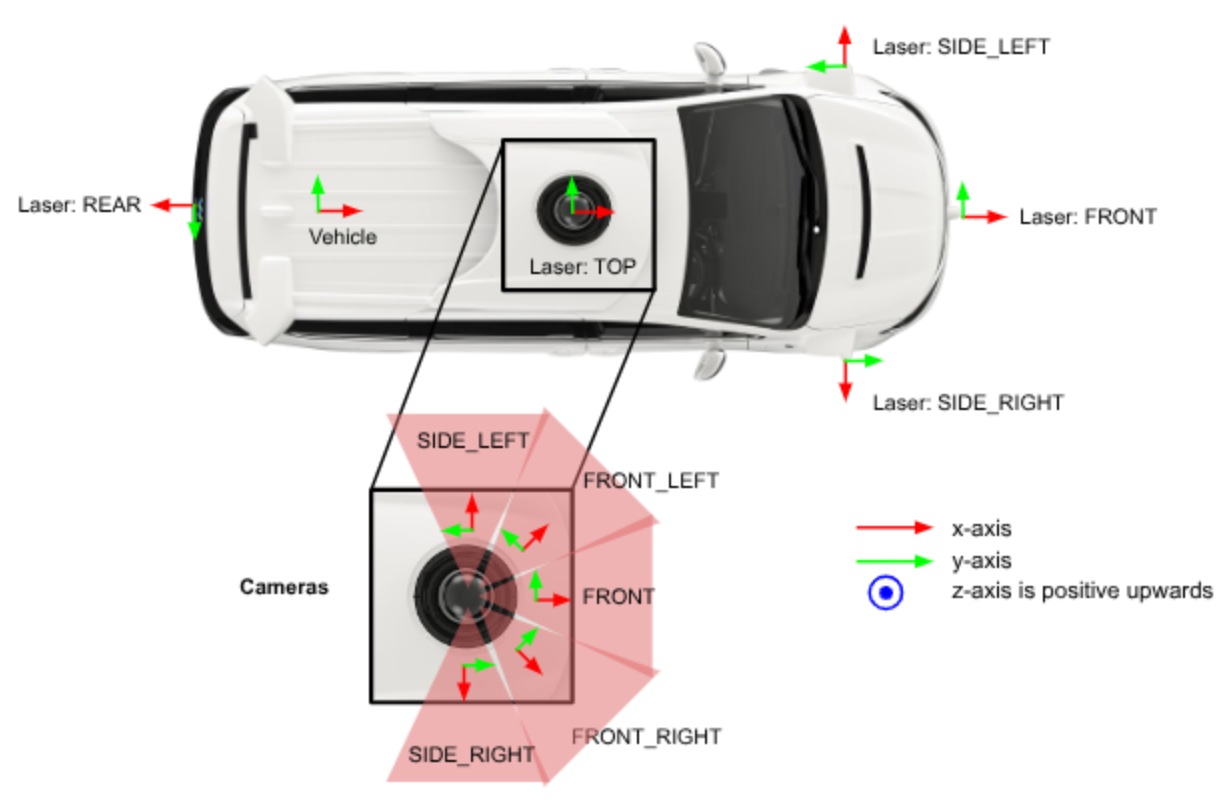
\includegraphics[scale=0.25]{gambar/wopd_sensors.png}
  \caption{Sensor layout and coordinate systems, WOPD}
  \label{fig:wopd_sensors}
\end{figure}

\begin{figure}[H]
  \centering
  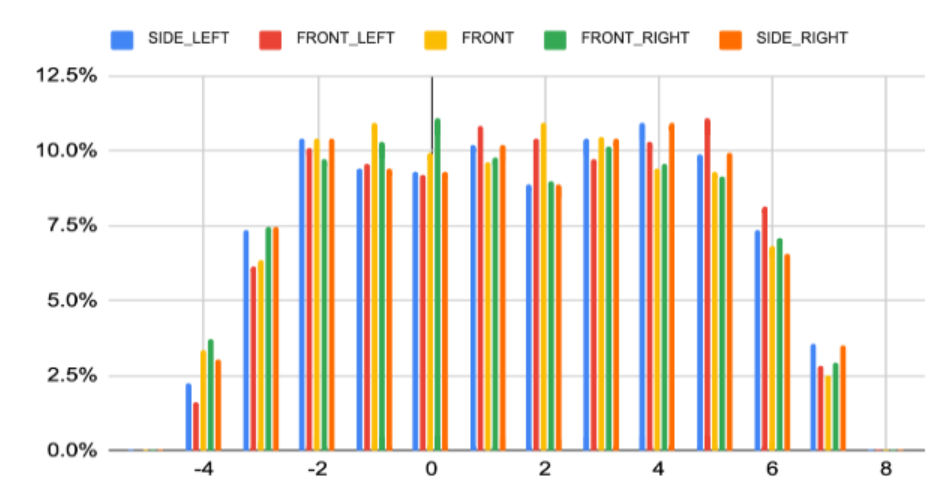
\includegraphics[scale=0.4]{gambar/sensor_sync.png}
  \caption{Camera-LiDAR synchronization accuracy}
  \label{fig:sensor_sync}
\end{figure}

\subsection{NVIDIA DRIVE and \emph{Edge Computing} in Autonomous Vehicles}

The implementation of \emph{Edge Computing} in autonomous vehicles relies entirely on high-performance computing hardware installed within the vehicle. This hardware, often referred to as the "brain" of the vehicle, must be capable of processing data from dozens of sensors and running complex AI algorithms within milliseconds. This hardware is fundamentally different from cloud server computers, as it must operate within strict constraints of power, heat, and size inside the vehicle, while also meeting very high automotive safety standards (ASIL – \emph{Automotive Safety Integrity Level}).

The NVIDIA DRIVE platform is one of the most dominant in the autonomous vehicle market. This platform is \emph{scalable}, ranging from basic ADAS functions to full autonomous driving capabilities (Level 4/5).

\begin{enumerate}[nolistsep]
    \item Hardware: The flagship platform at the time of this report is DRIVE Orin, a System-on-Chip (SoC) capable of delivering up to 254 trillion operations per second (TOPS).
    \item Implementation: Automakers such as Mercedes-Benz~\parencite{nvidia_mercedes_av}, Volvo~\parencite{nvidia_volvocars2025}, and Jaguar Land Rover~\parencite{nvidia_jlr2022} use the NVIDIA DRIVE platform to power their ADAS and autonomous driving systems. Mercedes-Benz, for example, uses DRIVE Orin for its Level 3 DRIVE-PILOT system.
\end{enumerate}


\subsection{NVIDIA Jetson and Development of Autonomous Vehicle Systems}

NVIDIA Jetson is a series of computer computing modules integrated with a GPU and CPU that can be used for developing autonomous vehicle systems~\parencite{proxpc2024jetson}. The main differences and specific roles of Jetson in the context of autonomous system development are:

\begin{enumerate}[nolistsep]
    \item Accessibility: Although still considered relatively expensive in Indonesia, platforms such as the Jetson Nano Developer Kit or Jetson AGX Orin Developer Kit are significantly more accessible to universities, startups, or research teams compared to the automotive-grade DRIVE platform. Researchers can experiment with perception algorithms, sensor fusion, and motion planning on the Jetson platform without requiring large investments or industrial partnerships. Many small-scale autonomous vehicles, delivery robots, and competition-oriented autonomous vehicles are powered by Jetson modules.
    \item Flexibility: Jetson modules allow for flexible prototyping and iterative development, making them ideal for testing custom software stacks or integrating new sensors. They support a wide range of AI frameworks and toolkits provided by NVIDIA, such as TensorRT, CUDA, and DeepStream.
\end{enumerate}

% \subsection{Hukum Newton}

% % Contoh penggunaan referensi dari pustaka
% Newton pernah merumuskan \parencite{Newton1687} bahwa \lipsum[8]
% % Contoh penggunaan referensi dari persamaan
% Kemudian menjadi persamaan seperti pada persamaan \ref{eq:FirstLaw}.

% % Contoh pembuatan persamaan
% \begin{equation}
%   % Label referensi dari persamaan yang dibuat
%   \label{eq:FirstLaw}
%   % Baris kode persamaan yang dibuat
%   \sum \mathbf{F} = 0\; \Leftrightarrow\; \frac{\mathrm{d} \mathbf{v} }{\mathrm{d}t} = 0.
% \end{equation}

% \lipsum[9]

% \subsection{Anti Gravitasi}

% \lipsum[10]

\section{Evaluation Metrics}

The proposed RT-LIVO2DM framework is assessed along two orthogonal dimensions: \emph{perception quality} and \emph{temporal performance}. To assess perception quality, we shall use the mAPH metric, which is computed as such: 

Assume each object class $c\in\mathcal{C}$ (vehicles, pedestrians, cyclists, \emph{etc.}) we first compute Average Precision (AP$_c$).  
Let  
\[
\mathcal{D}_c=\{(b_i, s_i)\}_{i=1}^{N_c}
\]  
denote the set of predicted 3-D bounding boxes $b_i$ with associated confidence scores $s_i$, and  
\[
\mathcal{G}_c=\{g_j\}_{j=1}^{M_c}
\]  
the ground-truth boxes for that class.  
A prediction is a \emph{true positive} if its 3-D Intersection-over-Union (IoU) with some unmatched ground-truth box exceeds the dataset-specific threshold $\tau$ (Waymo uses $\tau=0.5$).  
Sorting $\mathcal{D}_c$ by decreasing score yields the precision-recall curve  
\[
P(R)=\frac{\text{TP}(R)}{\text{TP}(R)+\text{FP}(R)},
\qquad
R=\frac{\text{TP}(R)}{M_c},
\]  
and  
\[
\text{AP}_c=\int_0^1 P(R)\,dR.
\]  
The \emph{mean} over classes is  
\[
\text{mAP}= \frac{1}{|\mathcal{C}|}\sum_{c\in\mathcal{C}}\text{AP}_c.
\]

Waymo additionally penalises mis-aligned orientations.  
For every matched pair $(b_i,g_j)$ let $\Delta\theta_{ij}$ be the absolute yaw-angle difference.  
The \emph{heading-weight} is  
\[
w_{ij}= \min\!\left(1,\ \frac{180^\circ-\Delta\theta_{ij}}{180^\circ}\right).
\]  
Each true positive contributes $w_{ij}$ instead of $1$ when computing TP, giving a weighted precision $P_{\text{H}}(R)$ and hence a weighted AP$_c^{\text{H}}$.  
The class-mean is denoted  
\[
\text{mAPH}= \frac{1}{|\mathcal{C}|}\sum_{c\in\mathcal{C}}\text{AP}_c^{\text{H}}.
\]

To assess temporal performance, we shall use the latency/inference time metric along with FPS (frames per second), which are computed as such:

The latency $T_{\text{inf}}$ is the wall-clock time between presenting a synchronized (LiDAR+image) frame to the system and receiving the final 3-D bounding-box list.  
Formally, for a validation set of $N$ frames,

\[
T_{\text{inf}}= \frac{1}{N}\sum_{k=1}^{N}t_k \quad[\text{ms}],
\qquad
t_k = t_{\text{end},k}-t_{\text{start},k}.
\]

The reciprocal of mean latency, clipped to the hardware’s sustained throughput, is

\[
\text{FPS}= \frac{1000}{T_{\text{inf}}} \quad[\text{Hz}].
\]

% Precision measures the proportion of predicted bounding boxes that are true positives:

% \begin{equation}
% \text{Precision} = \frac{\text{True Positives}}{\text{True Positives} + \text{False Positives}}.
% \end{equation}

% In the context of 3D object detection, a prediction is considered a true positive if its 3D Intersection over Union (IoU) with the ground truth box exceeds a certain threshold (we shall set the default metric at 0.5 for this research). We report class-wise and average precision across various object types (e.g., vehicles, pedestrians, cyclists) and detection ranges.

% Inference time refers to the average time taken by the model to process a single frame and produce 3D bounding box predictions. It is measured in milliseconds (ms) and is computed over the entire validation/test set as:

% \begin{equation}
% \text{Inference Time (ms)} = \frac{\sum_{i=1}^{N} t_i}{N}
% \end{equation}

% where:
% \begin{itemize}
%     \item $t_i$ is the time taken to process the $i$-th frame,
%     \item $N$ is the total number of frames in the validation/test set.
% \end{itemize}

For experiment preparation purposes, this research will assume a perception system latency of below 40ms to be optimal, and any systems with inference time higher than 40ms to be marked as non-capable of real-time inference. However, RT-LIVO2DM will not be designed with a target of 40ms inference time. Rather, it will be designed with a target of as low of an inference time as possible, evaluated on the same hardware (Jetson AGX ORIN) under different computational load scenarios. 
  \cleardoublepage

  % Konten metodologi
  \chapter{METHODOLOGY}

\section{System Design}

\begin{figure}[H]
  \centering
  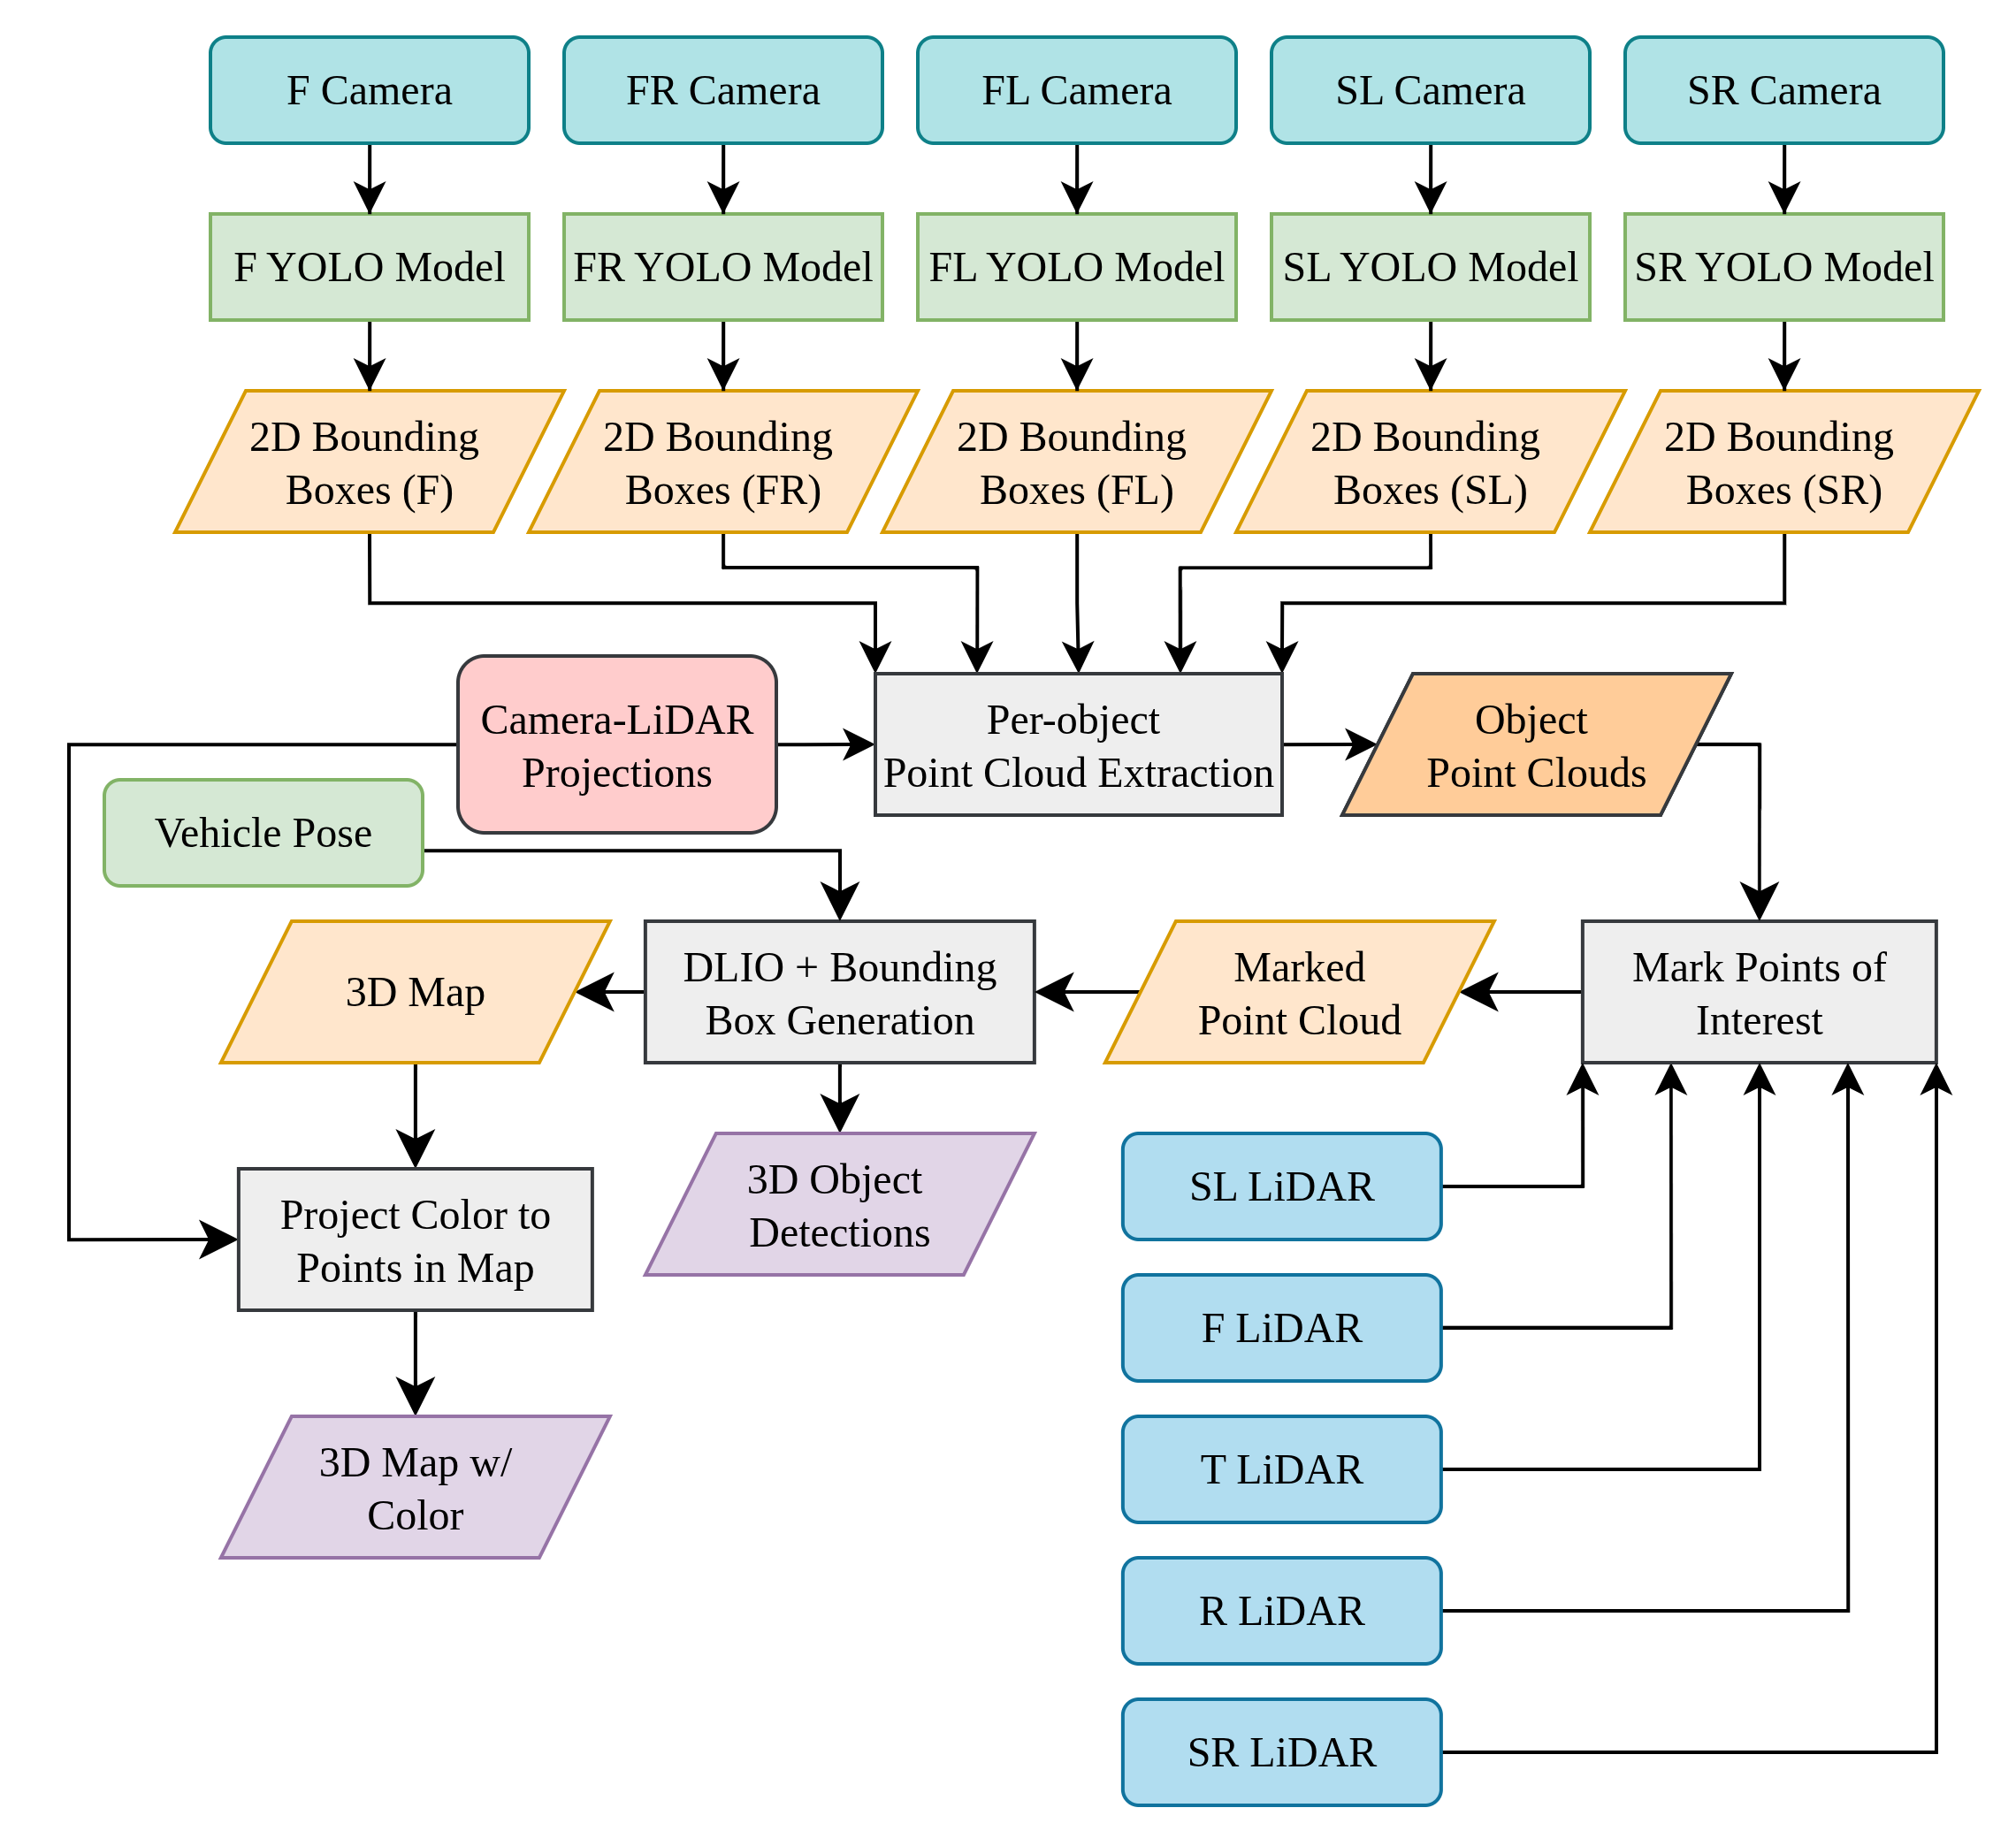
\includegraphics[scale=0.15]{gambar/rt_livo2dm_full.png}
  \caption{Proposed architecture for RT-LIVO2DM}
  \label{fig:rt_livo2dm_full}
\end{figure}

Figure~\ref{fig:rt_livo2dm_full} shows the proposed architecture of the RT-LIVO2DM system. RT-LIVO2DM combines 2D detection results from each camera angle with LiDAR projections to create 3D bounding box detections and a color 3D map.

\subsection{Shard Acquisition and Preprocessing}
In the Waymo Open Perception Dataset, a shard is a single, self-contained TFRecord file that packages a contiguous slice of the original driving log—typically 20–30 seconds of synchronized sensor data including LiDAR sweeps, camera images, IMU poses, and ground-truth labels. Instead of distributing one enormous file, the dataset is split into thousands of shards so researchers can download only the subset they need, stream them efficiently during training, or parallelize ingestion across multiple workers.

\subsection{Image Data Extraction}
After collecting the TFRecord shards, the images and labels are extracted and stored in a directory. The directory structure will follow the standard YOLO format for training, with a subdirectory for each camera.

\subsection{Modeling: 2D Object Detection}
Five different instances of the YOLOv11 model will be trained, one for each viewpoint. Each camera recording will be processed using a YOLOv11 model that has been specifically trained for that viewpoint. This approach is based on the known limitation of the YOLO algorithm, whish is its \emph{tendency} to achieve higher accuracy for each class in the \emph{testing dataset} when the class appears in positions similar to those in the \emph{training dataset}. Therefore, the author aims to prevent \emph{underfitting} caused by overly generalized learning that can occur when training a single model on data from all viewpoints. Since WOPD encompasses a huge range of scenarios for each viewing angle, the available training data for each camera is sufficient for this approach.

In WOPD, each 2D image is represented in the \((u, v, c)\) format, where \(u\) and \(v\) denote the horizontal and vertical pixel coordinates within the image frame, and \(c\) is the camera index. This format is used for the Camera-LiDAR projection available in WOPD, which will convert the \((u, v, c)\) data into a 3D point relative to the vehicle.

\subsection{Modeling: Per-Object Point Cloud Extraction}

\begin{figure}[H]
  \centering
  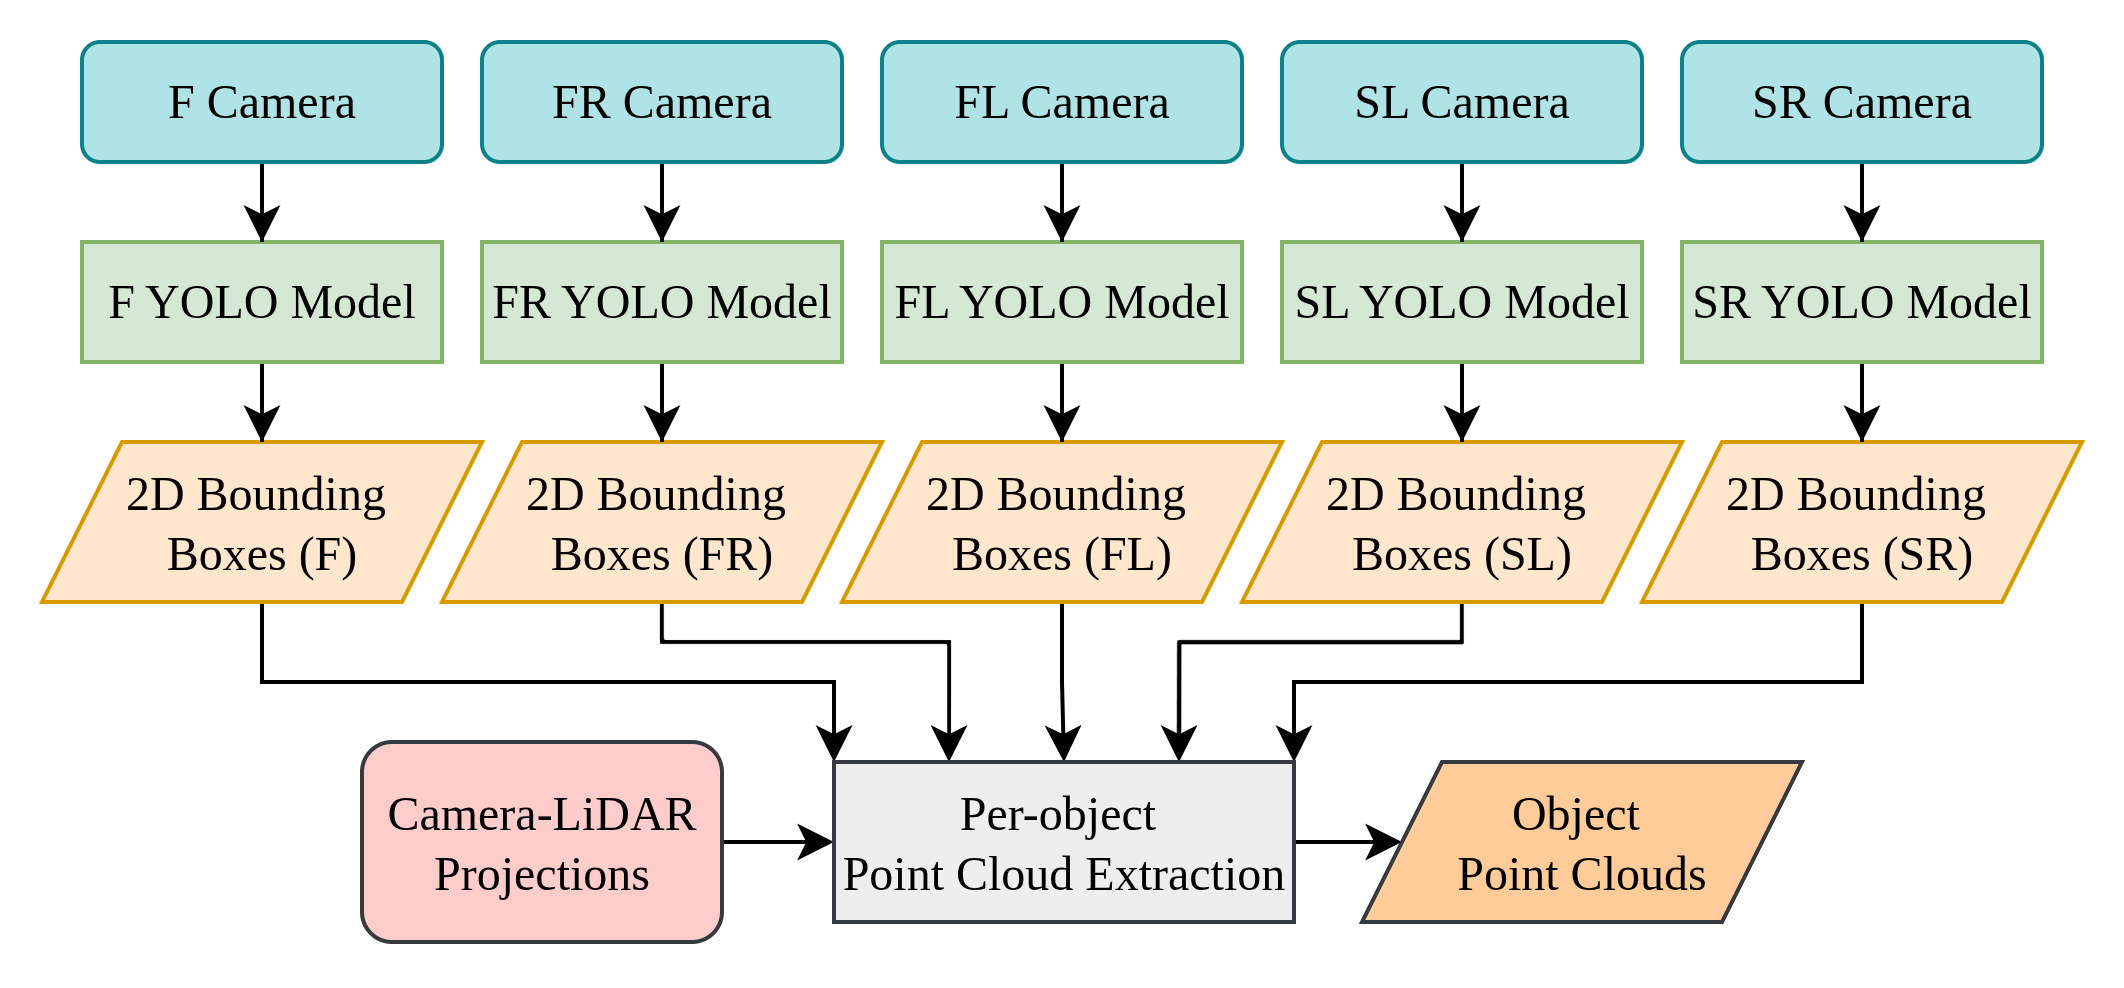
\includegraphics[scale=0.2]{gambar/object_pc.png}
  \caption{Process flow, gathering point clouds for each object}
  \label{fig:object_pc}
\end{figure}

Camera-LiDAR projections available with WOPD will be utilized to convert 2D bounding-box images into 3D Point Clouds for each object, as visualized by Figure~\ref{fig:object_pc}. This process is to be done by matching every pixel corresponding to the 2D object (every pixel inside the bounding box of a certain object in the image) into its corresponding LiDAR points. Then, to eliminate any background or foreground objects overlapping with the bounding box from the point cloud, the points' distance from the LiDAR is taken into account and those that fall outside percentiles \verb|min_p| and \verb|max_p| are discarded. Values for \verb|min_p| and \verb|max_p| are to be determined from a lightweight Artificial Neural Network (ANN), taking account the 2D inference class to produce a clean lidar point cloud for each object. 

\subsection{Modeling: 3D Bounding Box Generation}

\begin{figure}[H]
  \centering
  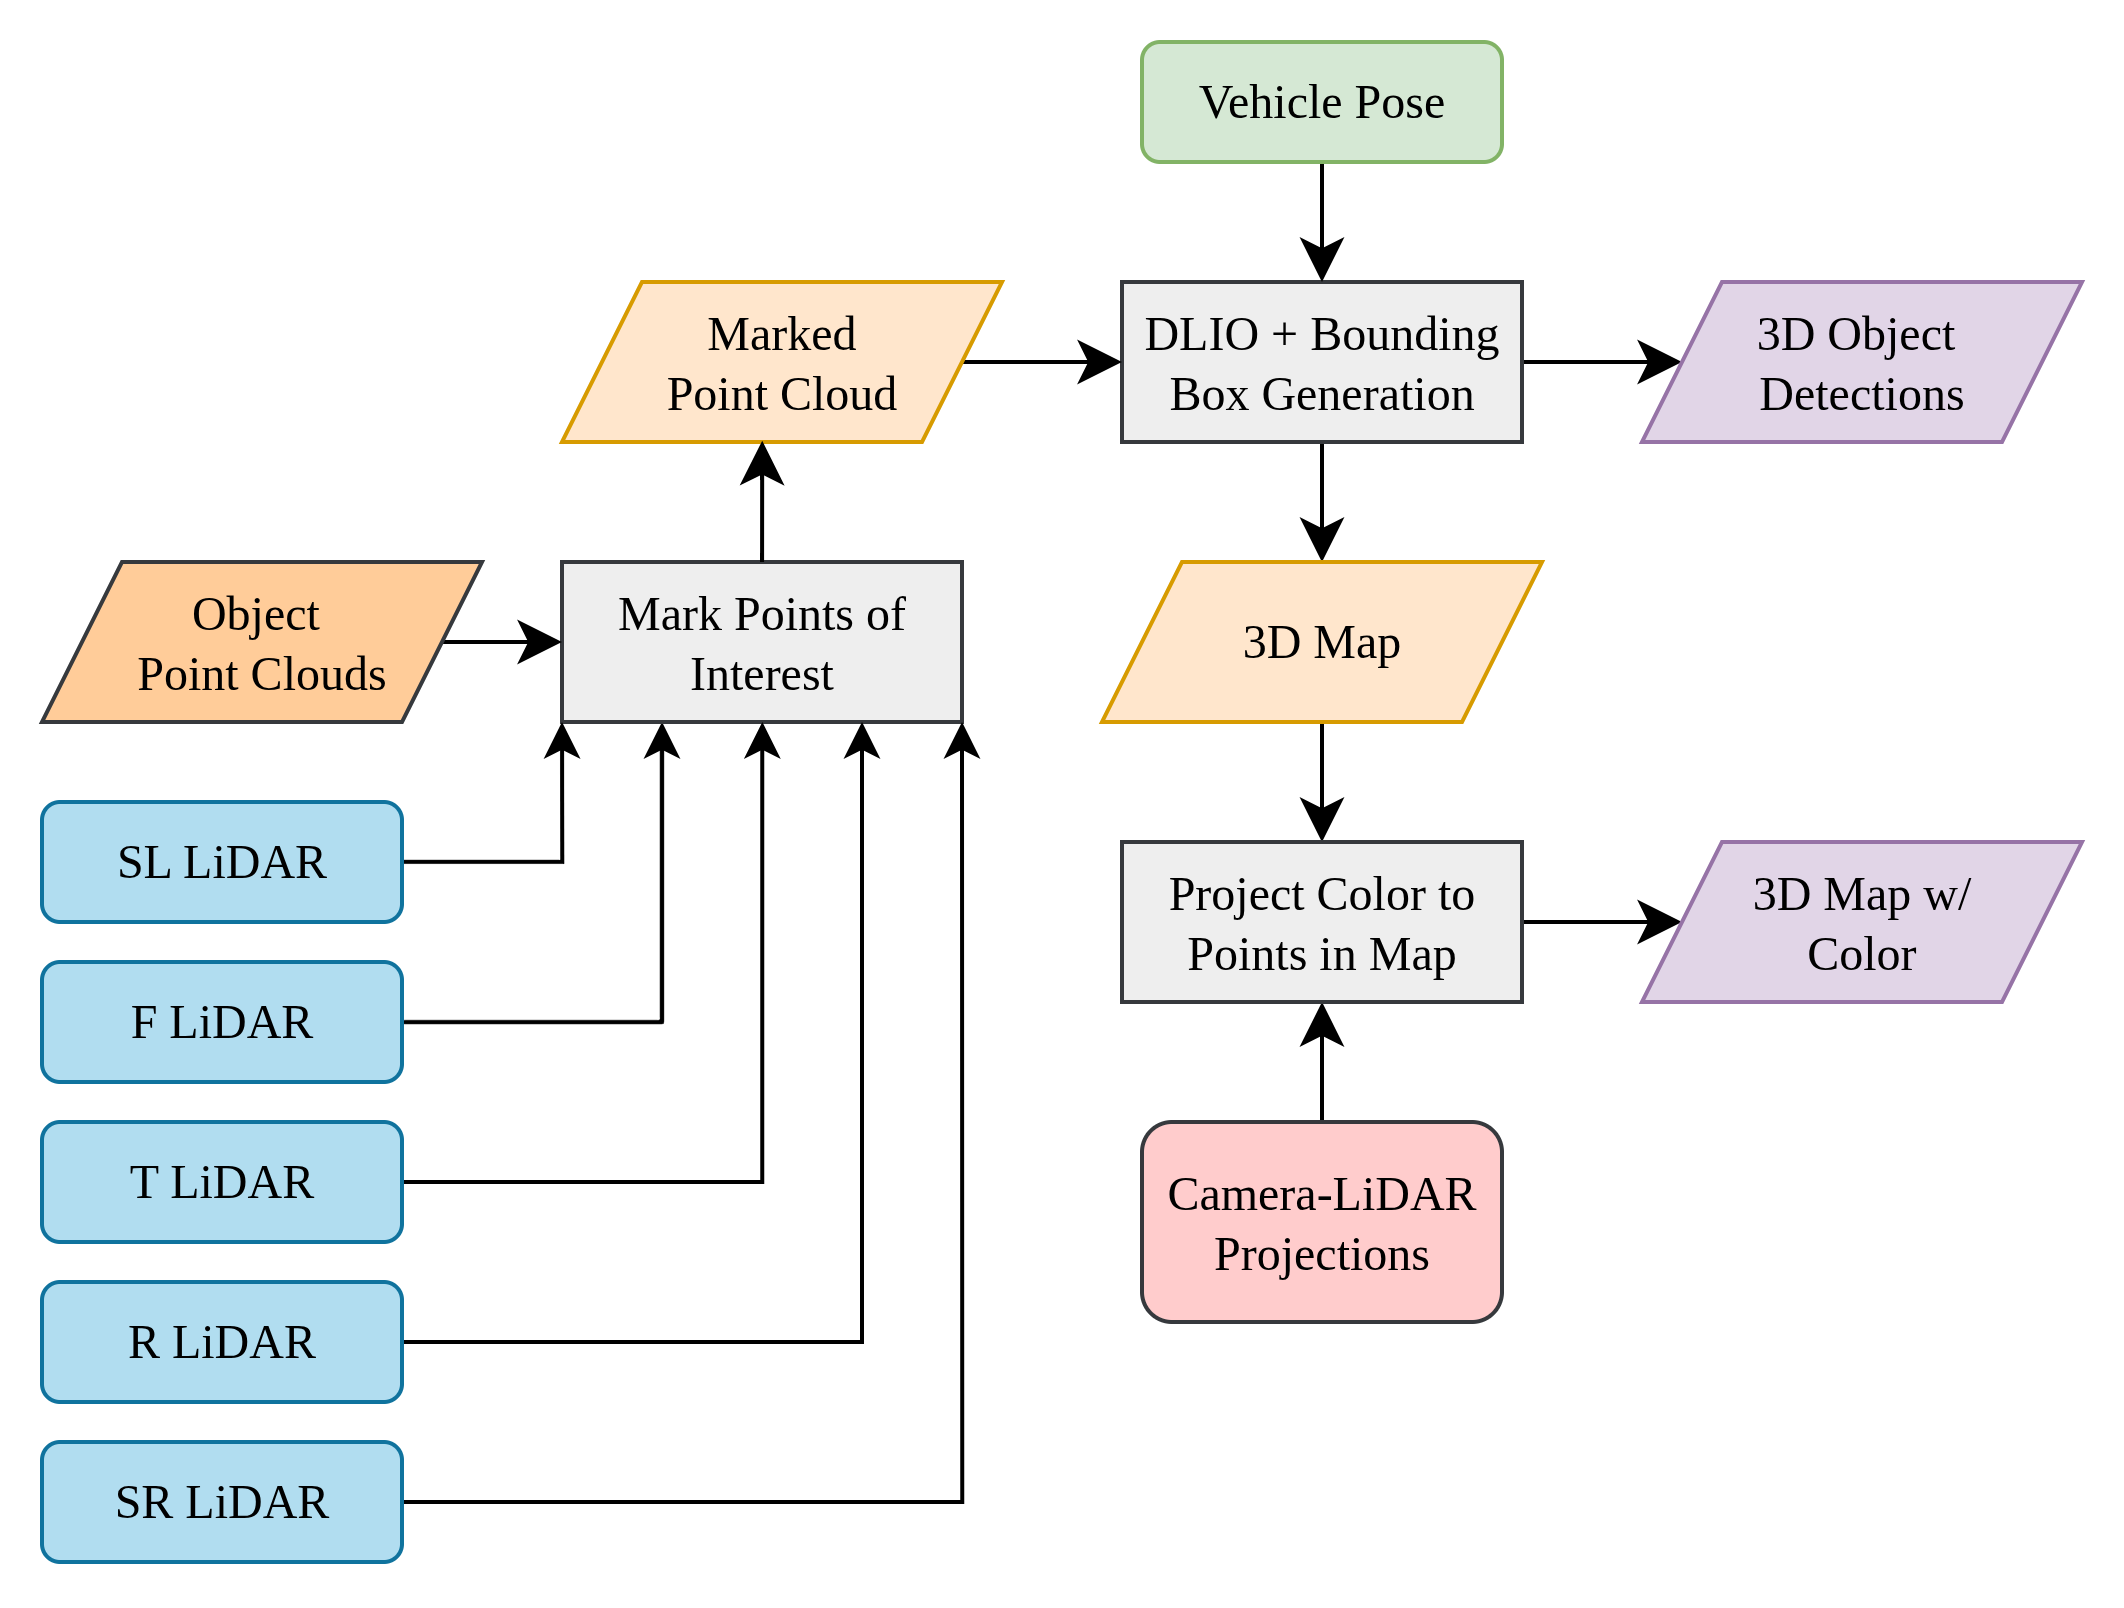
\includegraphics[scale=0.2]{gambar/detection_and_mapping.png}
  \caption{Modeling: 3D Object Detection and Mapping}
  \label{fig:detection_and_mapping}
\end{figure}

A combination between the lidar point cloud itself and vehicle pose data will be combined in order to create a high-precision 3D Map. The LiDAR point cloud data will be segmented using concave-hull and convex-hull K-Nearest Methods to extract reference objects (\emph{objects of interest}) from the environment. Changes in the orientation and position of each reference object will be used to estimate location changes. The IMU in this system serves to add context to the \emph{pose} transition between two instances of point cloud detection, improving the accuracy of orientation and position estimation for each object of interest. Figure~\ref{fig:detection_and_mapping} shows the process flow.

\section{Hardware Environment}

\subsection{NVIDIA AD103-400} 

\begin{figure}[H]
  \centering
  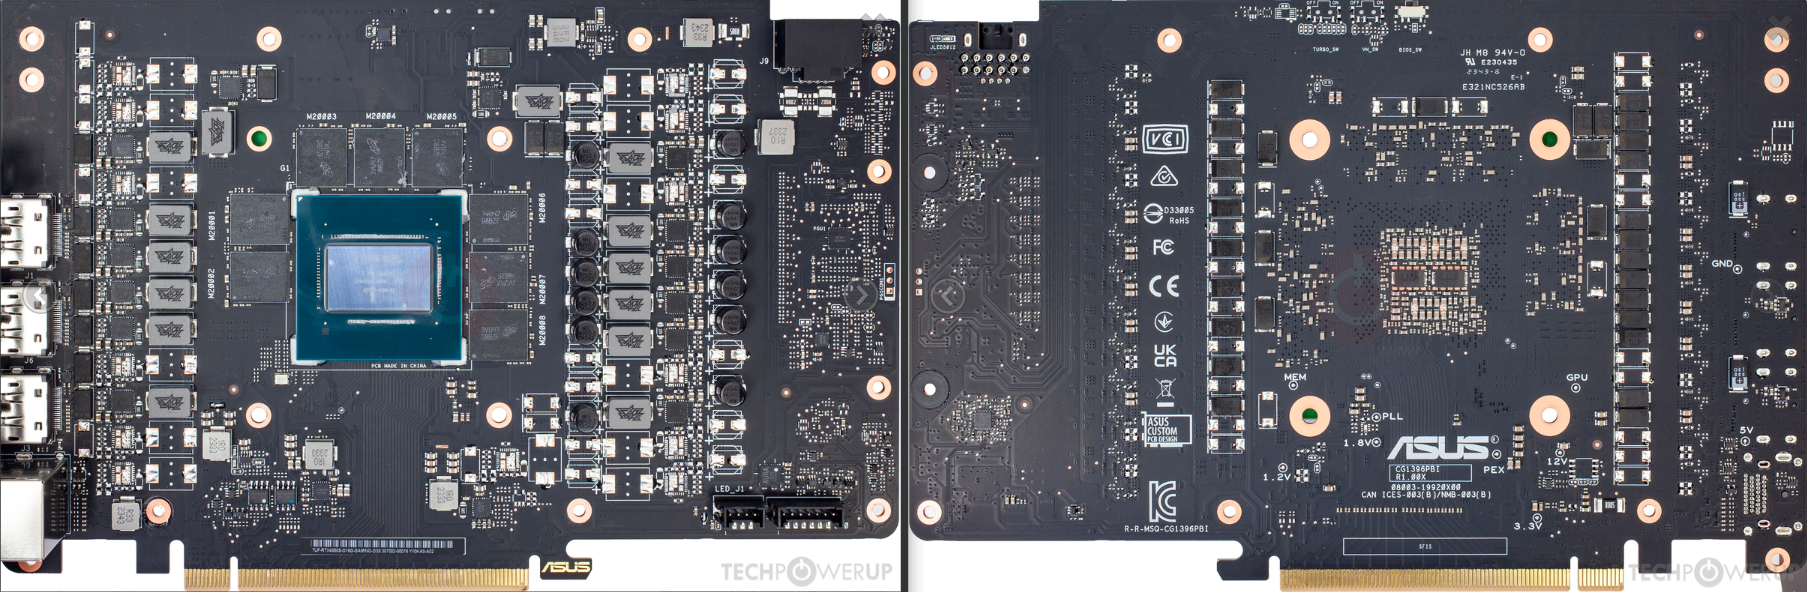
\includegraphics[scale=0.23]{gambar/ad103_400.png}
  \caption{Front view (left) and back view (right) of the NVIDIA AD103-400 GPU with ASUS-manufactured PCB}
  \label{fig:ad103_400}
\end{figure}

The NVIDIA AD103-400, commonly known as the RTX 4080 Super, is a consumer-grade GPU from NVIDIA. Due to its relative ease-of-access and significant computational capacity. The AD103-400 on an ASUS-manufactured motherboard (shown in Figure~\ref{fig:ad103_400}) will be used for training the multiple YOLO models as well as the lightweight ANN models used in RT-LIVO2DM. Table~\ref{tab:ad103_specifications} describes the specification of the AS103-400 in detail.

\begin{table}[h!]
\centering
\caption{Specifications of the NVIDIA AD103-400}
\label{tab:ad103_specifications}
\begin{tabular}{lcc}
\toprule
\textbf{Attribute} & \textbf{Value} \\
\midrule
GPU Model & NVIDIA AD103-400 \\
GPU Architecture & Ada Lovelace \\
CUDA Cores & 10,240 \\
Tensor Cores & 320 \\
Base Clock & 2.295 GHz \\
Boost Clock & 2.505 GHz \\
VRAM Capacity & 16 GB GDDR6X \\
Memory Interface Width & 256-bit \\
Memory Bandwidth & 736 GB/s \\
L2 Cache & 64 MB \\
TDP (Thermal Design Power) & 320 W \\
Compute Performance (FP32) & 52.22 TFLOPS \\
Manufacturing Process & TSMC 4N (4 nm) \\
\bottomrule
\end{tabular}
\end{table}

\subsection{NVIDIA Jetson AGX ORIN} 

\begin{figure}[H]
  \centering
  \includegraphics[scale=0.1]{gambar/jetson_agx_orin.png}
  \caption{NVIDIA Jetson AGX ORIN: with casing (left) and without casing (right)}
  \label{fig:jetson_agx_orin}
\end{figure}

NVIDIA Jetson AGX ORIN (as shown in Figure~\ref{fig:jetson_agx_orin}) is one of the variants in the NVIDIA Jetson family. This research will use Jetson AGX ORIN as the testing platform due to its comparable computational scale with the NVIDIA DRIVE ORIN, which is widely used in modern autonomous vehicle applications. Table~\ref{tab:jetson_agx_orin_specifications} details the technical specifications of the NVIDIA Jetson AGX ORIN. The Jetson AGX ORIN is pre-built with capabilities for hardware-wise down-throttling of computational capacity, making it a preferrable choice for inference hardware for this research, by consistently emulating different computational capacity scenarios.

\begin{table}[h!]
  \centering
  \caption{Specifications of the NVIDIA Jetson AGX Orin}
  \label{tab:jetson_agx_orin_specifications}
  \begin{tabular}{lcc}
  \toprule
  \textbf{Specification} & \textbf{Value} \\
  \midrule
  Processor & 12-core ARM Cortex-A78AE v8.2 64-bit CPU \\
  CUDA Cores & 2,048 \\
  Tensor Cores & 64 \\
  Memory & 64 GB LPDDR5  \\
  Storage & 64 GB eMMC 5.1 \\
  Memory Bandwidth & 204.8 GB/s \\
  AI Performance (INT8) & Up to 275 TOPS \\
  AI Performance (FP16) & Up to 137 TFLOPS \\
  Power Consumption & 15 W – 60 W (configurable) \\
  Networking & 10/100/1000 BASE-T Ethernet \\
  Form Factor & 100 mm × 87 mm \\
  Operating System & Ubuntu-based JetPack SDK \\
  \bottomrule
  \end{tabular}
\end{table}

\section{Implementation Approach}

\subsection{Data Extraction}
Algorithm~\ref{prog:waymo_get} outlines the process of developing a minimal reproducible workflow for downloading a \emph{training} or \emph{validation} shard.

\begin{algorithm}[H]
\caption{Minimal Workflow to Acquire and Inspect a Waymo Open Perception Shard}
  \label{prog:waymo_get}
  \begin{algorithmic}[1]
  \Require Internet connection, \texttt{gsutil}, Python~$\geq$3.8, TensorFlow~$\geq$2.11
  \Ensure Local directory \texttt{./wopd/training/} containing n shards and a verified frame count

  \State \textbf{Environment}:
  \State \quad \texttt{pip install waymo-open-dataset-tf-2-11-0} \Comment{or latest tag}

  \State \textbf{Select shards}:
  \State \quad $S \gets$ list of any n files matching 

  \texttt{gs://.../individual\_files/training/segment-*.tfrecord}

  \State \textbf{Download}:
  \State \quad \texttt{gsutil -m cp} $S$ \texttt{./wopd/training/}

  \State \textbf{Sanity check}:
  \State \quad $L \gets$ \texttt{glob("./wopd/training/segment-*.tfrecord")}
  \State \quad $D \gets$ \texttt{tf.data.TFRecordDataset}$(L)$
  \State \quad \textbf{print} ``Num. frames:'' $\sum_{\_ \in D} 1$
  \end{algorithmic}
\end{algorithm}

\subsection{Image Data Extraction}

Algorithm~\ref{prog:offline_extract} describes the outline of converting the collected shard/s into a directory of JPEG files and a manifest JSON file to be used for training purposes. The exact directory structure will follow the standard YOLO format for training.

\begin{algorithm}[H]
  \caption{Offline Pre-extraction (Training Mode)}
  \label{prog:offline_extract}
  \begin{algorithmic}[1]
  \Require List of shards $\mathcal{S}$, target camera $c$ (e.g. \texttt{FRONT})
  \Ensure Directory \texttt{./images/} of JPEG files and \texttt{manifest.json}

  \State $\mathcal{M} \gets [\;]$ \Comment{Empty JSON manifest}
  \For{shard $f \in \mathcal{S}$}
      \For{$(\text{img}, K, \text{labels})$ from \Call{FrameParser}{$f, c$}}
          \State $\text{frame\_id} \gets$ unique identifier from $f$
          \State write\_jpeg(img, \texttt{"./images/\{frame\_id\}.jpg"})
          \State $\mathcal{M}.\text{append}\bigl(\{\text{"file": } \ldots,\ \text{"labels": } \ldots\}\bigr)$
      \EndFor
  \EndFor
  \State flush\_json($\mathcal{M}$, \texttt{"manifest.json"})
  \end{algorithmic}
\end{algorithm}

% \begin{algorithm}[H]
% \caption{Online Streaming (Validation / Live Demo)}
% \label{prog:online_stream}
% \begin{algorithmic}[1]
% \Require List of shards $\mathcal{S}$, target camera $c$
% \Ensure Infinite generator of pre-processed RGB tensors

% \Function{waymo\_stream}{$\mathcal{S}, c$}
%     \For{shard $f \in \mathcal{S}$}
%         \For{$(\text{img}, \_, \_)$ from \Call{FrameParser}{$f, c$}}
%             \State $\text{tensor} \gets$ \Call{preprocess\_for\_yolo}{img} \Comment{resize, normalize, etc.}
%             \State \textbf{yield} tensor
%         \EndFor
%     \EndFor
% \EndFunction
% \end{algorithmic}
% \end{algorithm}

\subsection{Modeling: 2D Object Detection}

Algorithm~\ref{prog:yolo_loop} outlines the process of running a minimal YOLO inference loop on a running Waymo shard. The function \Call{waymo\_stream}{$\mathcal{S}, c$} is a generator that returns pre-processed RGB tensors from a shard. 

\begin{algorithm}[H]
\caption{Minimal YOLO Inference Loop}
\label{prog:yolo_loop}
\begin{algorithmic}[1]
\Require Trained YOLO model $\mathcal{M}$, generator \Call{waymo\_stream}{$\mathcal{S}, c$}
\Ensure Per-frame predictions $\mathcal{R}_t$

\State load $\mathcal{M} \gets$ \texttt{"yolov11n.pt"}
\For{tensor $T_t$ from \Call{waymo\_stream}{$\mathcal{S}, \text{"FRONT"}$}}
    \State $\mathcal{R}_t \gets$ \Call{predict}{$\mathcal{M}, T_t, \text{device="cuda:0"}$}
    \State \Call{post\_process}{$\mathcal{R}_t$} \Comment{project to 3D, log, etc.}
\EndFor
\end{algorithmic}
\end{algorithm}

\subsection{Modeling: Per-Object Point Cloud Extraction}

Algorithm~\ref{alg:pepce} describes the process flow of extracting per-object point cloud as a step in RT-LIVO2DM inference in detail.

\begin{algorithm}[H]
\caption{Per-object Point Cloud Extraction}
\label{alg:pepce}
\begin{algorithmic}[1]
\Require Set of 2D bounding boxes $\mathcal{B}$ (F, FR, FL, SL, and SR 2D Bounding Boxes) \\
         Lidar-camera projection function $P: (u, v, c) \rightarrow \mathbb{R}^3$ \\
         Pretrained ANN model $M$ for min/max percentile prediction
\Ensure Set $\mathcal{P}$ of refined 3D point clouds (one point cloud per bounding box)

\State $\mathcal{P} \gets \{\}$ \Comment{Initialize result set of point clouds}

\ForAll{bounding box $b_i \in \mathcal{B}$}
    \State $C_i \gets$ camera index where $b_i$ is detected
    \State $P_i \gets \{\}$ \Comment{Initialize point set for this box}
    \ForAll{pixels $(u, v)$ within $b_i$}
        \State $p \gets P(u, v, C_i)$ \Comment{Project pixel to 3D}
        \If{$p$ is valid}
            \State $P_i \gets P_i \cup \{p\}$
        \EndIf
    \EndFor

    \State $c_i \gets$ class label of detection $b_i$
    \State $d_i \gets$ distances of all points in $P_i$ to ego-vehicle

    \Comment{Use ANN model to determine percentiles based on class}
    \State $(\text{min}_p, \text{max}_p) \gets M(P_i, c_i)$
    \Comment{$M$ takes class label as input, returns two percentiles}

    \State $d_{\text{min}} \gets \text{percentile}(d_i, \text{min}_p)$
    \State $d_{\text{max}} \gets \text{percentile}(d_i, \text{max}_p)$

    \State $P_i \gets \{p \in P_i \mid d_{\text{min}} \leq \|p\| \leq d_{\text{max}}\}$
    \State $\mathcal{P} \gets \mathcal{P} \cup \{P_i\}$ \Comment{Append result}
\EndFor

\State \textbf{Output:} $\mathcal{P}$, a set of refined 3D point clouds per detected object
\end{algorithmic}
\end{algorithm}

\subsection{Modeling: 3D Bounding Box Generation}

Point cloud data from WOPD LiDAR sensors will be marked with an object label to determine which object (if any) each point belongs to. A modification of DLIO will be implemented to convert the marked point cloud into both 3D Bounding Boxes for each object and a 3D Map. The point cloud of each object will undergo a function involving Convex Hull + Minimum Volume Bounding Box to determine its corresponding 3D bounding box. This approach is similar to how one of the subsystems in DLIO (mentioned later) works, which allows for the segmentation of 3D objects from point cloud data without the need for significant computational resource. Algorithm~\ref{alg:3dbbox} describes the process in detail.

\begin{algorithm}[H]
  \caption{3D Bounding Box Generation}
  \label{alg:3dbbox}
  \begin{algorithmic}[1]
  \Require Point cloud $\mathcal{P}$ as a list of 3D points
  \Ensure Center $C$, Size $S$, Rotation matrix $R$
  \State Initialize empty point cloud object: $\mathcal{P}_{cd} \gets \texttt{PointCloud()}$
  \State Assign point data: $\mathcal{P}_{cd}.\texttt{points} \gets \texttt{Vector3dVector}(\mathcal{P})$
  \State Compute oriented bounding box: $\mathcal{B} \gets \mathcal{P}_{cd}.\texttt{get\_oriented\_bounding\_box}()$
  \State Extract center: $C \gets \mathcal{B}.\texttt{center}$
  \State Extract extent: $S \gets \mathcal{B}.\texttt{extent}$
  \State Extract rotation: $R \gets \mathcal{B}.\texttt{R}$
  \State \Return $C, S, R$
  \end{algorithmic}
\end{algorithm}
  \cleardoublepage

  % Konten lainnya
  \chapter{EXPECTED RESULTS}

\section{Expected Results of the Research}

A comparative analysis between the RT-LIVO2SM approach and existing methods is expected to demonstrate that RT-LIVO2SM can deliver advantageous outcomes in real-time object detection scenarios when compared to existing methods.

\section{Preliminary Results}

\sloppy
Preliminary research has uncovered that Waymo Open Dataset preferrable for benchmarking the performance of the RT-LIVO2SM system, due to the large number of previous implementations that have published their performance results using this dataset. Communication with the Robotics team at ITS, specifically Team Barunastra ITS, has been done regarding the potential provisioning of the NVIDIA Jetson AGX Orin Developer Kit for performance testing. Additionally, practical unlimited access to the computational capabilities of the NVIDIA AD103-400 for model training during the research period has been secured, ensuring minimal disruptions in model training.

As a footnote, the researcher already has experience in performing \emph{debugging} and \emph{tweaking} on the DLIO architecture \parencite{dlio}. With approximately two years of active experience in dataset collection and processing for \emph{Computer Vision} via the Roboflow platform—gained during their time as a \emph{Perceptions Programmer} for the Barunastra ITS robotics team—the researcher has also experimented with the YOLOv5, YOLOv7, YOLOv8, YOLOv9, YOLOv10, and YOLOv11 architectures. This background gives the researcher confidence in augmenting the capabilities of both DLIO and YOLO architectures by integrating them into the proposed RT-LIVO2SM architecture.

  \cleardoublepage

  \chapter{RESEARCH SCHEDULE}

\newcommand{\w}{}
\newcommand{\G}{\cellcolor{gray}}
\begin{table}[H]
  \captionof{table}{Timeline Table}
  \label{tbl:timeline}
  \begin{tabular}{|p{3.5cm}|c|c|c|c|c|c|c|c|c|c|c|c|c|c|c|c|}

    \hline
    \multirow{2}{*}{Activity} & \multicolumn{16}{|c|}{Week}                                                                       \\
    \cline{2-17}              &
    1                         & 2                             & 3  & 4  & 5  & 6  & 7  & 8  & 9  & 10 & 11 & 12 & 13 & 14 & 15 & 16 \\
    \hline

    Data Processing           &
    \G                        & \G                            & \w & \w & \w & \w & \w & \w & \w & \w & \w & \w & \w & \w & \w & \w \\
    \hline

    Model Training            &
    \w                        & \w                            & \G & \G & \G & \G & \G & \G & \G & \G & \G & \w & \w & \w & \w & \w \\
    \hline

    Data Analysis             &
    \w                        & \w                            & \w & \w & \w & \w & \G & \G & \G & \G & \G & \G & \w & \w & \w & \w \\
    \hline

    Research Evaluation       &
    \w                        & \w                            & \w & \w & \w & \w & \w & \w & \w & \w & \G & \G & \G & \G & \G & \G \\
    \hline
  \end{tabular}
\end{table}

As shown in the timeline in Table~\ref{tbl:timeline}, most of the research duration will be allocated to training the models for each camera angle. Data analysis is expected to begin in week 7, once a portion of the trained models are ready for comparison and evaluation. This timeline also anticipates potential adjustments to training parameters based on insights gained from model analysis.

  \cleardoublepage

  % Daftar pustaka
  \chapter*{BIBLIOGRAPHY}
  \addcontentsline{toc}{chapter}{BIBLIOGRAPHY}
  \renewcommand\refname{}
  \vspace{2ex}
  \renewcommand{\bibname}{}
  \begingroup
    \def\chapter*#1{}
    \printbibliography
  \endgroup


\end{document}
